% Note: Multiple abstract versions below - select one for final submission
% % Abstract, take 1
% % This paper demonstrates how to quantify uncertainty in regression models through a novel classification and clustering transform, enabling safety-critical autonomous systems to determine when predictions should not be trusted. While prior work has addressed regression uncertainty through Bayesian methods, ensemble techniques, and distributional predictions, these approaches typically require architectural modifications or computational overhead. We present an alternative approach that transforms regression problems into classification tasks, then leverages the geometric properties of the classification space to quantify uncertainty. By using k-means clustering on the softmax outputs of correctly classified examples we determine class centroids. The distance from new predictions to these centroids provides a principled uncertainty measure that requires no model retraining. We validate this approach on autonomous vehicle steering control in the CARLA simulator, where both CNN and Vision Transformer models are trained for steering angle prediction. By quantizing continuous steering angles into discrete bins, we show that distances to class centroids increase monotonically with visual perturbations (RGB pepper noise) and correlate linearly with lane invasion risk. Our method successfully predicts lane invasions before they occur by monitoring sequential predictions that exceed distance thresholds, enabling timely handover to human control. This classification-based uncertainty quantification offers a practical, computationally efficient alternative to existing methods while providing interpretable safety guarantees for regression-based autonomous systems.

% % Abstract, take 2
% % This paper demonstrates how to quantify uncertainty in regression via a classification and clustering transform. Prior work on regression uncertainty quantification (UQ) has primarily relied on Bayesian methods, ensembles, parametric distributions, or conformal prediction to estimate predictive variances and decompose epistemic/aleatoric sources (e.g., Gawlikowski et al., 2021; Lakshminarayanan et al., 2016; Zhou et al., 2025). While effective in domains like autonomous driving and medical imaging, these approaches often require architectural modifications or high computational overhead and lack direct, threshold-based confidence for sequential decision-making in safety-critical systems.

% % We propose a novel adaptation: quantizing continuous regression outputs (e.g., steering angles) into discrete classes, training classifiers, and seeding k-means centroids with softmax averages of correct predictions to define a bounded clustering space. Distances from new predictions to centroids serve as uncertainty proxies, with thresholds enabling "I don't know" flags for low-confidence cases.

% % We demonstrate a practical application in predicting lane invasions within a CARLA-simulated autonomous driving environment. Under increasing RGB pepper noise, centroid distances correlate linearly with lane deviations, allowing proactive detection of risky prediction sequences and timely handover to human control. Results show enhanced safety without eliminating all errors, generalizing to other regression-dependent systems like robotics or environmental forecasting. This method provides a lightweight, verifiable safety net for autonomous reliability.

% % Full title - for paper
% % When to Not Trust Your Regression Model: Quantifying Uncertainty for Autonomous System Safety

\chapter{Contribution 2 - Uncertainty Quantification in Regression Models via Classification and Clustering}

This chapter demonstrates how to quantify uncertainty in regression models through a novel classification and clustering transform, enabling safety-critical autonomous systems to determine when predictions should not be trusted. While prior work has addressed regression uncertainty through Bayesian methods, ensemble techniques, and distributional predictions, these approaches typically require architectural modifications or computational overhead. We present an alternative approach that transforms regression problems into classification tasks, then leverages the geometric properties of the classification space to quantify uncertainty. By using k-means clustering on the softmax outputs of correctly classified examples we determine class centroids. The distance from new predictions to these centroids provides a principled uncertainty measure that requires no model retraining. We validate this approach on autonomous vehicle steering control in the CARLA simulator, where both CNN and Vision Transformer models are trained for steering angle prediction. By quantizing continuous steering angles into discrete bins, we show that distances to class centroids increase monotonically with visual perturbations (RGB pepper noise) and correlate linearly with lane invasion risk. Our method successfully predicts lane invasions before they occur by monitoring sequential predictions that exceed distance thresholds, enabling timely handover to human control. This classification-based uncertainty quantification offers a practical, computationally efficient alternative to existing methods while providing interpretable safety guarantees for regression-based autonomous systems.

%%%%%%%%%%%%%%%%%%
%% INTRODUCTION %%
%%%%%%%%%%%%%%%%%%

\section{Introduction}

The deployment of machine learning models in autonomous systems has revolutionized fields ranging from self-driving vehicles to medical robotics, yet the critical question of when these systems should trust their own predictions remains largely unresolved. In safety-critical applications such as autonomous driving, medical diagnosis, and industrial automation, models must not only produce accurate predictions but also provide reliable estimates of their uncertainty (\cite{malinin2020regression, wibbeke2025evaluating, bigi2024prediction}). The consequences of overconfident predictions in such domains can be catastrophic, making uncertainty quantification not merely desirable but essential for safe autonomous operation (\cite{gawlikowski2021survey}).

Traditional regression models, while powerful for continuous prediction tasks, inherently lack mechanisms for expressing confidence in their outputs. Standard neural networks, for instance, provide only point estimates without any indication of prediction reliability (\cite{gawlikowski2021survey}). This limitation becomes particularly problematic in autonomous systems operating in dynamic, unpredictable environments where the model may encounter scenarios significantly different from its training distribution. Without proper uncertainty quantification, autonomous systems cannot make informed decisions about when to rely on model predictions, when to seek human intervention, or when to engage fail-safe mechanisms.

Existing approaches to uncertainty quantification in regression have made significant strides in addressing these challenges. Bayesian neural networks attempt to model parameter uncertainty by maintaining distributions over network weights rather than point estimates (\cite{dunger2025uncertainties}). Ensemble methods create multiple models with different initializations or training subsets, using the variance across predictions as an uncertainty measure (\cite{dunger2025uncertainties}). Monte Carlo dropout techniques approximate Bayesian inference by applying dropout during inference, generating multiple predictions to estimate uncertainty. Deep ensembles and evidential learning frameworks have also emerged as promising approaches for regression uncertainty quantification (\cite{wibbeke2025evaluating}).

However, these existing methods face several limitations that hinder their adoption in autonomous systems. Bayesian approaches, while theoretically principled, often suffer from computational overhead that makes real-time inference challenging (\cite{anand2025uncertainty}). Ensemble methods require training and maintaining multiple models, multiplying computational and memory requirements. Many uncertainty quantification techniques also struggle with calibration issues, where the predicted confidence levels do not accurately reflect true prediction reliability (\cite{gawlikowski2021survey}). Furthermore, the uncertainty estimates produced by these methods are often difficult to interpret, making it challenging for autonomous systems to translate uncertainty measures into actionable decisions.

The regulatory and safety requirements for autonomous systems demand not only accurate uncertainty estimates but also interpretable and computationally efficient methods that can operate within strict real-time constraints. Current approaches often fail to meet these dual requirements of accuracy and efficiency, creating a significant gap between theoretical advances in uncertainty quantification and practical deployment needs in autonomous systems.

\textbf{Regression-to-Classification Transformation}

An alternative approach to direct regression uncertainty quantification involves transforming continuous prediction problems into discrete classification tasks. This transformation, known as regression via classification (RvC), has gained significant attention in machine learning as it often improves model performance compared to standard regression approaches (\cite{stewart2022regression, berg2020deep}). The fundamental principle involves discretizing the continuous target variable into a finite set of non-overlapping bins or intervals, effectively converting the regression problem into a multi-class classification task (\cite{torgo1996regression, torgo1997regression}).

The transformation process requires careful consideration of how to partition the continuous output space. The most common approaches include \textbf{equal-width binning}, where the continuous range is divided into intervals of equal length, and \textbf{quantile-based binning}, where bins are created to contain approximately equal numbers of training examples (\cite{berg2020deep, barkov2024efficient}). More sophisticated methods employ adaptive quantization schemes that consider the underlying data distribution, with different strategies proving suitable for balanced data (linear quantization), long-tailed distributions (logarithmic quantization), or highly imbalanced scenarios (adaptive quantization) (\cite{xiong2023deep}).

The choice of discretization strategy creates a fundamental trade-off between classification accuracy and discretization error. Too few bins result in large quantization errors when recovering continuous target values, while too many bins lead to insufficient training examples per class, potentially degrading classification performance (\cite{berg2020deep}). Advanced approaches address this challenge through techniques such as kernel density integral quantization, which adaptively interpolates between uniform and quantile-based strategies (\cite{mccarter2024unmasking}), and optimal binning methods that satisfy constraints such as maintaining minimum samples per bin or enforcing monotonicity (\cite{huang2022mbct}).

Once classification is performed, the continuous regression estimate is typically recovered by computing the expected value over the predicted class probabilities weighted by bin centers or through more sophisticated distributional approaches (\cite{barkov2024efficient, keren2018calibrated}). This transformation approach has demonstrated particular success in computer vision tasks such as depth estimation, age estimation, and crowd counting, where classification formulations often outperform direct regression (\cite{fu2018deep, xiong2023deep}).

The regression-to-classification paradigm offers several advantages relevant to uncertainty quantification in autonomous systems. Classification models naturally provide probability distributions over discrete outcomes, which can serve as confidence measures. The discrete nature of the output space enables clearer decision boundaries and more interpretable confidence thresholds. Additionally, the vast arsenal of classification techniques, including ensemble methods and calibration approaches, becomes available for the transformed problem (\cite{guha2024conformal, pintea2023step}).

However, traditional regression-to-classification approaches still face limitations in autonomous system contexts. The binning process introduces discretization artifacts and requires careful hyperparameter tuning. The recovered continuous estimates may not adequately capture the uncertainty structure needed for safety-critical decisions. Most importantly, existing approaches do not provide principled methods for determining when the transformed model's predictions should be trusted or rejected in real-time autonomous operation.

This paper addresses these limitations by proposing a novel approach that transforms regression problems into classification tasks, then employs clustering techniques with centroid-based thresholds to provide computationally efficient and interpretable uncertainty estimates. Our method offers several key advantages: (1) computational efficiency suitable for real-time autonomous operation, (2) interpretable uncertainty measures based on geometric distance to learned cluster centroids, and (3) clear decision boundaries that enable autonomous systems to determine when predictions should be trusted or rejected.

The remainder of this paper is organized as follows: Section 2 reviews related work in uncertainty quantification for regression, Section 3 presents our clustering-based approach, Section 4 evaluates the method on benchmark datasets and autonomous system scenarios, and Section 5 concludes with implications for autonomous system safety and future research directions.

%%%%%%%%%%%%%%%%
% RELATED WORK %
%%%%%%%%%%%%%%%%

\section{Related Work}

This section reviews existing approaches to uncertainty quantification in regression models, with particular emphasis on methods relevant to autonomous systems. We organize our discussion around four key areas: traditional uncertainty quantification methods for regression, regression-to-classification transformation approaches, uncertainty estimation in classification models, and applications in safety-critical autonomous systems.

\textbf{Bayesian Approaches}

Bayesian neural networks (BNNs) represent one of the most principled approaches to uncertainty quantification in regression. Rather than learning point estimates for network parameters, BNNs maintain probability distributions over weights, enabling the model to express uncertainty about both parameters and predictions \cite{dunger2025uncertainties}. The predicted distribution directly contains probabilistic information that can be used for uncertainty estimation, providing a theoretically sound framework for distinguishing between aleatoric (data) and epistemic (model) uncertainty \cite{gawlikowski2021survey}.

However, BNNs face significant practical limitations, particularly in autonomous system deployments. The computational overhead associated with sampling from parameter distributions or performing variational inference makes real-time inference challenging \cite{anand2025uncertainty}. Additionally, the choice of prior distributions and approximation schemes can significantly impact the quality of uncertainty estimates, often requiring domain expertise and extensive hyperparameter tuning \cite{gawlikowski2021survey}.

\textbf{Ensemble Methods}

Ensemble approaches address uncertainty quantification by training multiple models with different initializations, data subsets, or architectural variations. The variance across ensemble predictions serves as an uncertainty measure, with higher variance indicating greater prediction uncertainty \cite{dunger2025uncertainties}. Deep ensembles, in particular, have demonstrated strong performance across various regression tasks by combining the predictions of multiple neural networks trained independently \cite{wibbeke2025evaluating}.

While ensemble methods often provide well-calibrated uncertainty estimates, they suffer from significant computational and memory overhead. Training and maintaining multiple models multiplies resource requirements, making deployment in resource-constrained autonomous systems problematic \cite{malinin2020regression}. Furthermore, ensemble methods primarily capture epistemic uncertainty through model diversity but may not adequately represent aleatoric uncertainty inherent in the data distribution.

\textbf{Monte Carlo Methods}

Monte Carlo dropout approximates Bayesian inference by applying dropout during both training and inference phases. By performing multiple forward passes with different dropout patterns, the method generates a distribution of predictions that can be used to estimate uncertainty \cite{wibbeke2025evaluating}. This approach offers a computationally efficient alternative to full Bayesian inference while maintaining some theoretical grounding.

Despite its efficiency advantages, Monte Carlo dropout has been shown to produce poorly calibrated uncertainty estimates, particularly when the dropout rate is not properly tuned for the specific task \cite{gawlikowski2021survey}. The method also struggles to capture epistemic uncertainty effectively when the model is confident but potentially wrong, a critical limitation for safety-critical applications.

\textbf{Evidential Learning}

Evidential deep learning frameworks attempt to learn the parameters of probability distributions directly, rather than learning point estimates. These methods place distributions over the parameters of the predictive distribution, enabling the quantification of epistemic uncertainty through the concentration of evidence \cite{malinin2020regression}. For regression tasks, evidential approaches often model the target distribution using parameterized families such as Gaussian or Student-t distributions.

While evidential methods show promise in providing interpretable uncertainty measures, they often require careful initialization and training procedures to avoid pathological solutions. The reliance on specific distributional assumptions may also limit their applicability to complex, multi-modal target distributions common in real-world autonomous system scenarios \cite{bigi2024prediction}.

% Next we examine regression-to-classification Transformation.

\textbf{Binning and Discretization Strategies}

The transformation of regression problems into classification tasks through discretization has a long history in machine learning, with early foundational work establishing the theoretical basis for this approach \cite{torgo1996regression, torgo1997regression}. The core challenge lies in effectively discretizing continuous target variables into meaningful bins that preserve the underlying structure while enabling effective classification.

\textbf{Equal-width binning} divides the continuous range into intervals of equal length, providing a simple and interpretable discretization scheme \cite{berg2020deep, barkov2024efficient}. However, for skewed distributions, this approach can result in bins with vastly different numbers of training examples, potentially leading to class imbalance issues that degrade classification performance.

\textbf{Quantile-based binning} addresses this limitation by creating bins that contain approximately equal numbers of training examples, ensuring balanced class distributions \cite{berg2020deep, barkov2024efficient}. While this approach improves classification balance, it may not respect the natural structure of the target distribution, potentially grouping dissimilar values together.

More sophisticated \textbf{adaptive quantization schemes} consider the underlying data distribution when determining bin boundaries. Different strategies prove suitable depending on the data characteristics: linear quantization for balanced data, logarithmic quantization for long-tailed distributions, and adaptive approaches for highly imbalanced scenarios \cite{xiong2023deep}. Advanced methods like kernel density integral quantization (KDI) adaptively interpolate between uniform and quantile-based strategies, automatically selecting appropriate discretization based on local data density \cite{mccarter2024unmasking}.

\textbf{Optimal Binning with Constraints}

Recent work has focused on developing principled approaches to binning that satisfy domain-specific constraints. Optimal binning methods use optimization techniques to maximize information-theoretic measures while respecting constraints such as minimum samples per bin, monotonicity requirements, or maximum number of bins \cite{huang2022mbct}. Mixed-integer programming approaches have been employed to identify optimal binning strategies that maximize measures like Jeffreys' Divergence, which reflects how well the discretized variable differentiates between classes \cite{barkov2024efficient}.

These constrained optimization approaches often provide superior discretization schemes compared to heuristic methods, but they introduce additional computational complexity and hyperparameter selection challenges. The trade-off between discretization quality and computational efficiency becomes particularly important in real-time autonomous system applications.

\textbf{Recovery Methods}

Once classification is performed on discretized targets, the continuous regression estimate must be recovered from the predicted class probabilities. The most common approach computes the expected value over predicted class probabilities weighted by bin centers or midpoints \cite{barkov2024efficient, keren2018calibrated}. More sophisticated recovery methods model the distribution within each bin, using training set statistics to refine the final continuous estimate.

Advanced recovery techniques include distributional approaches that maintain probability mass functions over bin boundaries, enabling more nuanced continuous predictions \cite{keren2018calibrated}. However, these methods may not significantly improve performance over simpler weighted averaging approaches, particularly when discretization is coarse.

% \subsection{Uncertainty Estimation in Classification}

\textbf{Calibration Methods}

The transformation from regression to classification enables the use of well-established classification uncertainty methods, but these require careful calibration to provide meaningful confidence estimates. Platt scaling, temperature scaling, and isotonic regression represent common post-hoc calibration techniques that adjust classifier outputs to better reflect true prediction confidence \cite{keren2018calibrated}.

\textbf{Bayesian binning} methods provide more sophisticated calibration by modeling the relationship between predicted probabilities and true frequencies using Bayesian inference \cite{huang2022mbct}. These approaches can capture complex calibration relationships but require additional validation data and computational overhead for training the calibration mappings.

\textbf{Conformal prediction} methods provide distribution-free uncertainty quantification by constructing prediction sets that contain the true target with a specified probability \cite{guha2024conformal}. Recent work has extended conformal prediction to regression-as-classification settings, enabling the construction of prediction intervals for continuous targets through the transformed classification framework.

The appeal of conformal methods lies in their theoretical guarantees: under the exchangeability assumption, conformal prediction sets achieve the desired coverage probability regardless of the underlying data distribution or model choice. However, the quality of prediction sets depends heavily on the choice of conformity scores and the effectiveness of the underlying classification model \cite{guha2024conformal}.

\textbf{Safety-Critical Requirements}

Autonomous systems operating in safety-critical environments require uncertainty quantification methods that satisfy stringent reliability, interpretability, and real-time performance requirements \cite{bigi2024prediction, wibbeke2025evaluating}. Traditional uncertainty methods often fail to meet these requirements due to computational overhead, calibration issues, or lack of interpretable confidence measures.

The automotive industry, in particular, has driven research into practical uncertainty quantification methods that can operate within the strict latency and reliability constraints of autonomous driving systems. Medical robotics and industrial automation present similar challenges, where prediction confidence directly impacts safety-critical decision making \cite{malinin2020regression}.

\textbf{Interpretability and Decision Making}

A critical limitation of many existing uncertainty quantification methods is their lack of interpretability, making it difficult for autonomous systems to translate uncertainty estimates into actionable decisions \cite{gawlikowski2021survey}. Rule-based systems for determining when to trust model predictions, when to seek human intervention, or when to engage fail-safe mechanisms require uncertainty measures that can be easily thresholded and interpreted by system designers.

Recent work has emphasized the need for uncertainty quantification methods that provide not just confidence estimates but also explanations for why particular predictions should or should not be trusted \cite{pintea2023step}. This requirement has driven interest in geometric and distance-based uncertainty measures that can be directly related to training data characteristics and model behavior.

\textbf{Motivation}

While existing uncertainty quantification methods provide valuable theoretical foundations and practical tools, they exhibit limitations such as computational complexity, Interpretability and the lack of a decision framework that hinder deployment in autonomous systems.

Our proposed clustering-based approach addresses these limitations by providing computationally efficient, interpretable uncertainty estimates based on geometric distance measures. By leveraging the regression-to-classification framework with centroid-based thresholds, our method enables clear decision boundaries for autonomous system safety while maintaining the computational efficiency required for real-time operation.

%%%%%%%%%%%
% METHODS %
%%%%%%%%%%%

\section{Methods}

This section presents our clustering-based uncertainty quantification approach for autonomous vehicle steering prediction. We describe the mathematical foundations of our method, the regression-to-classification transformation process, and the experimental setup using the CARLA autonomous driving simulator. Our approach addresses the critical need for computationally efficient and interpretable uncertainty estimation in safety-critical autonomous systems.

\textbf{Problem Formulation}

Consider a neural network trained for steering angle prediction in autonomous driving, where the model maps camera images $\mathbf{x} \in \mathbb{R}^{H \times W \times C}$ to steering angles $y \in \mathbb{R}$. Traditional regression approaches output a single continuous value without confidence estimates. Our method transforms this regression problem into a classification task, then applies geometric clustering analysis to quantify prediction uncertainty.

Let $f_{\theta}: \mathbb{R}^{H \times W \times C} \rightarrow \mathbb{R}^K$ represent our transformed neural network with parameters $\theta$, where $K$ is the number of discrete steering angle bins. The network outputs logits $\mathbf{z} = f_{\theta}(\mathbf{x}) = (z_1, z_2, \ldots, z_K)$, which are converted to probabilities via the softmax function:

$$p_i = \frac{e^{z_i}}{\sum_{j=1}^{K} e^{z_j}}$$

The resulting probability vector $\mathbf{p} = (p_1, p_2, \ldots, p_K)$ satisfies $\sum_{i=1}^K p_i = 1$ and represents the model's confidence distribution across steering angle classes.

\textbf{Discretization Strategy}

The continuous steering angle space is discretized into $K$ discrete bins corresponding to specific angular ranges. For autonomous driving applications, we implement three binning schemes based on CARLA's normalized control space:

\textbf{3-bin scheme:} $\{-0.065, 0.0, 0.065\}$ (Left, Straight, Right)

\textbf{5-bin scheme:} $\{-0.065, -0.015, 0.0, 0.015, 0.065\}$ (Hard Left, Soft Left, Straight, Soft Right, Hard Right)

\textbf{15-bin scheme:} $\{-0.065, -0.055, \ldots, -0.005, 0.0, 0.005, \ldots, 0.055, 0.065\}$ (Fine-grained steering control)

The number of bins must be odd to ensure a center bin corresponding to straight driving ($0.0°$ steering angle). Each configuration (15, 5, or 3 bins) represents a range of approximately $\pm 4.5°$ of the vehicle's $\pm 70°$ steering range, sufficient for lane-following without lane invasion on the experimental circuit.

\textbf{Model Architecture Adaptation}

The neural network architecture is modified to support classification outputs. The final linear layer changes from mapping to $\mathbb{R}^1$ (single continuous output) to mapping to $\mathbb{R}^K$ (K discrete class outputs). The loss function transitions from Mean Squared Error (MSE) for regression:

$$\mathcal{L}_{\text{MSE}} = \frac{1}{n} \sum_{i=1}^{n} (y_i - \hat{y}_i)^2$$

to Cross-Entropy Loss for classification:

$$\mathcal{L}_{\text{CE}} = -\frac{1}{n} \sum_{i=1}^{n} \sum_{j=1}^{K} y_{i,j} \log(p_{i,j})$$

where $y_{i,j}$ is the one-hot encoded true class and $p_{i,j}$ is the predicted probability for class $j$.

\textbf{Continuous Value Recovery}

For autonomous driving control, continuous steering angles must be recovered from discrete class predictions. The class index maps directly to the corresponding steering angle label. For example, for a classifier trained on data where steering angles were separated into 5 bins, a softmax output with highest score at index 1 (where indices go from 0 to 4), the corresponding label is $-0.015$, applying left steering to the vehicle.

\textbf{Clustering-Based Uncertainty Quantification Mathematical Framework}

Our uncertainty quantification method operates in the probability simplex defined by softmax outputs. Each prediction $\mathbf{p}$ lies within the $(K-1)$-dimensional standard simplex:

$$\Delta^{K-1} = \{\mathbf{p} \in \mathbb{R}^K : p_i \geq 0, \sum_{i=1}^K p_i = 1\}$$

This geometric constraint ensures that all cluster centroids and predictions exist within a bounded space, with maximum Euclidean distance between any two points bounded by $\sqrt{2}$, independent of dimensionality $K$.

\textbf{Centroid Calculation}

We compute class-specific centroids $\mathbf{C} = \{\mathbf{c}_1, \mathbf{c}_2, \ldots, \mathbf{c}_K\}$ from correct training predictions. For each class $k$, the centroid is calculated as:

$$\mathbf{c}_k = \frac{1}{|T_k|} \sum_{\mathbf{p} \in T_k} \mathbf{p}$$

where $T_k = \{\mathbf{p}_i : \arg\max(\mathbf{p}_i) = k \text{ and prediction is correct}\}$ represents the set of all correct predictions for class $k$.

\paragraph{Algorithm 1: Centroid Calculation}
\begin{verbatim}
Input: correct_predictions (n × K matrix of softmax outputs)
Output: centroids (K × K matrix of class centroids)

1. Initialize centroids ← zeros(K, K)
2. For each class k = 0 to K-1:
3.   indices ← where(argmax(correct_predictions, axis=1) == k)
4.   centroid ← mean(correct_predictions[indices], axis=0)
5.   centroids[k] ← centroid
6. Return centroids
\end{verbatim}

\textbf{Threshold Determination}

As a first pass, decision thresholds are determined using incorrect predictions from the training set. For each class $k$, we calculate the minimum distance from incorrect predictions to the corresponding centroid:

$$\tau_k = \min_{\mathbf{p} \in F_k} \|\mathbf{p} - \mathbf{c}_k\|_2$$

where $F_k = \{\mathbf{p}_i : \arg\max(\mathbf{p}_i) = k \text{ and prediction is incorrect}\}$ represents the set of incorrect predictions that were classified as class $k$. Fine-tuning and optimal threshold setting remains domain dependent.

\paragraph{Algorithm 2: Threshold Calculation}
\begin{verbatim}
Input: incorrect_predictions (n × K matrix), distances (n × 1 vector), 
true_classes (n × 1 vector)
Output: thresholds (K × 2 matrix of [threshold, class] pairs)

1. Initialize thresholds ← zeros(K, 2)
2. For each class k = 0 to K-1:
3.   class_distances ← distances[where(true_classes == k)]
4.   threshold ← min(class_distances)
5.   thresholds[k] ← [threshold, k]
6. Return thresholds
\end{verbatim}

\textbf{Decision Rule}

For a new prediction $\mathbf{p}_{\text{new}}$, we calculate distances to all centroids and apply the decision rule:

$$d_k = \|\mathbf{p}_{\text{new}} - \mathbf{c}_k\|_2$$

$$\text{predicted\_class} = \arg\max(\mathbf{p}_{\text{new}})$$

$$\text{decision} = \begin{cases}
\text{ACCEPT} & \text{if } d_{\text{predicted\_class}} < \tau_{\text{predicted\_class}} \\
\text{REJECT} & \text{otherwise}
\end{cases}$$

This geometric approach provides interpretable uncertainty measures: predictions closer to training centroids are more trustworthy, while predictions far from centroids indicate potential out-of-distribution inputs or model uncertainty.

\textbf{CARLA Simulation Environment Experimental Setup}

We conduct experiments using CARLA 0.9.13 (Car Learning to Act), an open-source autonomous driving simulator built on Unreal Engine \cite{dosovitskiy17}. CARLA provides realistic urban environments with dynamic weather, traffic, and pedestrian conditions, enabling controlled experimentation for autonomous driving algorithms.

The simulation configuration uses the Town04 figure-of-eight circuit. The route consists of 28 road segments following lane ID –2 (the second lane left-to-right, right-hand traffic). The vehicle is equipped with a front-facing RGB camera, whose mounting position and orientation are configurable and typically set at 1.5 units of distance above (along z axis) and 1.8 units of distance ahead (along x axis) of the vehicle's centre (waypoint). Weather conditions such as cloudiness, precipitation, and fog are controllable, as well as number of cars and pedestrians. The simulation runs in synchronous mode to ensure deterministic execution steps.

\textbf{Dataset Generation}

The dataset generation process is based on waypoint navigation. The vehicle follows predefined waypoints extracted from the town map mesh, identified by road\_id and lane\_id attributes. The figure-of-eight circuit is composed of waypoints spaced at 1-unit intervals for regression tasks and 3-unit intervals for classification tasks.

The steering algorithm computes the angular difference between the vehicle’s current orientation and the target waypoint orientation. This difference is applied as a steering correction to maintain lane-following behaviour, as defined by

\[
\mathrm{steering\_angle} = \mathrm{atan2}(\mathrm{target\_y} - \mathrm{vehicle\_y}, \mathrm{target\_x} - \mathrm{vehicle\_x}) - \mathrm{vehicle\_heading}
\]

During data collection, the system records RGB camera images (cropped and resized to 200×66 pixels), steering angle labels embedded in timestamped filenames, ground truth safety distances (measured as the perpendicular distance to the lane centerline), and lane invasion events (a distance greater than 0.85 units indicates a lane invasion). Each complete circuit lap produces approximately 28,000 labeled image–steering pairs under synchronous execution mode.

\textbf{Image Preprocessing}

Images undergo spatial cropping to remove sky regions and the vehicle hood, retaining only the pixels from y-coordinates 210 to 480. The cropped images are then resized to 200×66 pixels using bilinear interpolation to conform to the NVIDIA architecture requirements \cite{bojarski2016end}. Finally, RGB images are converted to the YUV color space following established autonomous driving practices \cite{lecun2004dave}, as YUV representation offers better perceptual similarity to human vision and improved performance in computer vision applications.

\textbf{Dataset Variants}

The regression variants include three configurations: \textbf{Vanilla}, which uses raw camera images with continuous steering angle targets; \textbf{Segmented}, which overlays lane segmentation markers on the images; and \textbf{Segmented with Fiducials}, which combines lane segmentation with fiducial markers.

For the classification variants, datasets are generated for each binning scheme (3, 5, and 15 bins). Two versions are produced for each scheme: \textbf{Unbalanced}, which preserves the natural steering angle distribution where straight driving predominates, and \textbf{Balanced}, in which images from minority classes are randomly duplicated to achieve equal class distributions.


\textbf{Neural Network Architecture}

We implement the NVIDIA end-to-end learning architecture \cite{bojarski2016end} adapted for both regression and classification tasks:

The implemented model follows the NVIDIA end-to-end learning architecture \cite{bojarski2016end}, adapted for both regression and classification tasks. The network consists of five convolutional layers followed by three fully connected layers and a single output layer. The convolutional block progressively increases the number of filters from 24 to 64 across five layers, employing kernel sizes of 5×5 and 3×3 with ELU activations and stride configurations designed to extract hierarchical spatial features from input images.  

The fully connected block maps the flattened feature representation through layers of 100, 50, and 10 neurons, each using ELU activations and dropout regularization with a rate of 0.1 to reduce overfitting. The final output layer consists of one neuron for regression tasks or \(K\) neurons for classification, where \(K \in \{3, 5, 15\}\) corresponds to the number of steering angle bins.  

Training is performed using the Adam optimizer with a learning rate of \(1\times10^{-5}\) and a batch size of 64 samples. Data are split randomly into 80\% for training and 20\% for validation. Early stopping is applied after six epochs without improvement in validation loss, with a maximum of 100 epochs. All experiments are executed on an NVIDIA GPU with CUDA acceleration.

In addition to the NVIDIA end-to-end convolutional architecture, a Vision Transformer (ViT) model is employed for comparative evaluation. The ViT is used directly for classification tasks, producing discrete steering angle predictions according to the chosen binning scheme. For regression tasks, the same model is adapted by replacing the final classification head with a single linear output neuron, enabling continuous steering angle estimation. This adaptation allows direct validation of the ViT’s capability to predict continuous steering values alongside the CNN-based baseline.

\textbf{Evaluation Metrics}

For regression tasks, performance is evaluated using the Mean Absolute Error (MAE), defined as  
\[
\text{MAE} = \frac{1}{n}\sum_{i=1}^{n}|y_i - \hat{y}_i|,
\]
and the Mean Squared Error (MSE), defined as  
\[
\text{MSE} = \frac{1}{n}\sum_{i=1}^{n}(y_i - \hat{y}_i)^2.
\]

For classification tasks, the primary metric is accuracy, representing the percentage of correct class predictions, complemented by per-class precision and recall to account for imbalanced datasets.

Uncertainty quantification is assessed through several additional metrics: the Accept Rate, measuring the percentage of predictions above a confidence threshold; the Reject Rate, representing the percentage below it; the Safety Margin, defined as the average distance to the decision boundary for accepted predictions; and the Lane Invasion Rate, which captures the frequency of lane violations during autonomous operation.


\textbf{Safety Assessment}

Lane invasion detection involves real-time monitoring of the vehicle's position relative to lane boundaries. Perpendicular distances exceeding 0.85 CARLA units trigger lane invasion events, indicating potential safety violations.

Distance-based safety integrates clustering-based uncertainty quantification with geometric safety measures. Predictions exhibiting high uncertainty (i.e., large centroid distances) are found to correlate with increased lane invasion risk, thereby validating the safety relevance of the proposed uncertainty estimates.

Fail-safe mechanisms are implemented for cases in which predictions are rejected due to high uncertainty. In such situations, the system can execute predefined responses, such as maintaining the current steering angle, requesting human intervention, or engaging emergency lane-keeping assistance.

This comprehensive methodology provides a principled framework for uncertainty-aware autonomous driving, combining regression-to-classification transformation with geometric clustering analysis to enable safe, interpretable decision-making in real-time autonomous systems.

%%%%%%%%%%%%%%%%%%%%%%%%%%%%
%% RESULTS AND DISCUSSION %%
%%%%%%%%%%%%%%%%%%%%%%%%%%%%

\section{Results And Discussion}

%%%%%%%%%%%%%%%%%%%%%
% REGRESSION MODELS %
%%%%%%%%%%%%%%%%%%%%%

\textbf{Regression Models}
\begin{longtable}{@{}lllllll@{}}
\toprule
Model Name & Dataset & Train Loss & Eval Loss & MAE & O MAE & D MAE \\
\midrule
\endfirsthead
\toprule
Model Name & Dataset & Train Loss & Eval Loss & MAE & O MAE & D MAE \\
\midrule
\endhead
RegCNNCUFid & Cont Unbal w/ Fids & 0.0000 & 0.0000 & N/A & 0.0036 & 0.0461 \\
RegCNNCU & Continuous Unbal & N/A & N/A & N/A & 0.0033 & 0.0588 \\
RgrViTCU & Continuous Unbal & 0.0002 & 0.0001 & 0.0076 & 0.0076 & 0.0399 \\
\bottomrule
\caption{Regression Model Performance}
\label{results:table_regression_models}
\end{longtable}

Table~\ref{results:table_regression_models} reports the performance of three regression models trained on the continuous unbalanced dataset. The columns are as follows: Train Loss and Eval Loss refer to the mean squared error on the training and evaluation sets, respectively; MAE is the mean absolute error computed during training; O MAE is the mean absolute error calculated over the combined training and evaluation sets; and D MAE is the mean absolute lateral deviation of the simulated vehicle from the centerline, measured during autonomous driving in the Town04 figure-of-eight loop. Where N/A appears, the corresponding value was not recorded during training.

The RegCNNCUFid model incorporates fiducial markers as input and achieved a D MAE of 0.0461, with an O MAE of 0.0036. The RegCNNCU model, which uses the same architecture without fiducials, obtained a slightly lower O MAE (0.0033) but a higher D MAE (0.0588). The difference in D MAE between these two models is small and may be attributed to statistical noise, as both values remain well below the operational threshold of 0.85, beyond which lane invasion would occur.

The RgrViTCU model, based on a ViT architecture, yielded an O MAE of 0.0076 and the lowest D MAE among the three (0.0399). Since MAE values were not recorded for the CNN-based models, comparisons across all models using that column are not possible. All D MAE values are within the bounds of acceptable simulated driving behavior, and the differences observed do not approach the threshold of operational relevance.

%%%%%%%%%%%%%%%%%%%%%%%%%
% CLASSIFICATION MODELS %
%%%%%%%%%%%%%%%%%%%%%%%%%

\textbf{Classification Models}
\begin{longtable}{@{}llllllll@{}}
\toprule
Model Name & Dataset & T Acc & T Loss & V Acc & V Loss & O Acc & D MAE \\
\midrule
\endfirsthead
\toprule
Model Name & Dataset & T Acc & T Loss & V Acc & V Loss & O Acc & D MAE \\
\midrule
\endhead
ClsCNN3bB & 3-bin Bal & 83.16\% & 0.3797 & 83.02\% & 0.3808 & 83.36\% & 0.0365 \\
ClsCNN3bU & 3-bin Unbal & 86.97\% & 0.3129 & 87.14\% & 0.3110 & 87.36\% & 0.0466 \\
ClsCNN5bB & 5-bin Bal & 87.45\% & 0.3001 & 86.92\% & 0.2975 & 87.70\% & 0.0491 \\
ClsCNN5bU & 5-bin Unbal & 92.87\% & 0.1993 & 93.03\% & 0.1928 & 93.18\% & 0.0753 \\
ClsCNN15bB & 15-bin Bal & 48.01\% & 1.0744 & 47.81\% & 1.0598 & 48.01\% & 0.0162 \\
ClsCNN15bU & 15-bin Unbal & 73.76\% & 0.7241 & 75.34\% & 0.6839 & 75.11\% & 0.0194 \\
ClsViT3bB & 3-bin Bal & N/A & 0.1875 & 97.15\% & 0.0960 & 97.97\% & 0.0462 \\
ClsViT3bU & 3-bin Unbal & N/A & 0.2625 & 91.93\% & 0.2075 & 92.50\% & 0.0397 \\
ClsViT5bB & 5-bin Bal & N/A & 0.1317 & 97.54\% & 0.0766 & 97.77\% & 0.0454 \\
ClsViT5bU & 5-bin Unbal & N/A & 0.1985 & 94.05\% & 0.1590 & 94.97\% & 0.0666 \\
ClsViT15bB & 15-bin Bal & N/A & 0.4012 & 92.92\% & 0.1984 & 93.86\% & 0.0925 \\
ClsViT15bU & 15-bin Unbal & N/A & N/A & N/A & N/A & 76.55\% & 0.0844 \\
\bottomrule
\caption{Classification Model Performance: training and self-driving, with quantized balanced and unbalanced datasets. The first row shows data for a CNN classifier trained on a 3-bin dataset - steering angles -0.065 (-4.55 degrees), 0 and 0.065 (4.55 degrees). The training accuracy is 83.17\%, the training loss 0.3739, the validation accuracy 83.02\%, the validation loss 0.3808, the overall accuracy when training and validation datasets are combined is 83.36\%. The distance mean average error (DMAE) is 0.0365, this is the average distance between the optimal middle-of-the-lane path and the vehicle path}
\label{results:classifier_models_results_table}
\end{longtable}

Table~\ref{results:classifier_models_results_table} presents the results for CNN and ViT models that were converted from regression models to perform classification, under three quantization schemes—3, 5, and 15 steering angle bins—and using either balanced or unbalanced datasets. The columns are as follows: T Acc and T Loss denote training accuracy and training loss; V Acc and V Loss are validation accuracy and validation loss; O Acc represents the overall accuracy across the full dataset (training and validation combined); and D MAE is the mean absolute error of the vehicle’s lateral deviation from the centerline. Entries marked N/A indicate that the corresponding values were not recorded during training. The D MAE values were computed through inference: after training, each model was deployed to drive autonomously around the Town04 figure-of-eight track, and its average distance from the intended trajectory was measured.

Among the CNN classifiers, ClsCNN5bU (trained on the unbalanced 5-bin dataset) achieved the highest overall accuracy (93.18\%), making it the best-performing CNN model. While its D MAE was slightly higher (0.0753), this remains well below the threshold (0.85 units) beyond which the vehicle would cross into an adjacent lane—meaning the deviation is not operationally significant and may be attributed to statistical noise. For the ViT models, ClsViT3bB (trained on the balanced 3-bin dataset) showed the strongest performance, with an overall accuracy of 97.97\% and a D MAE of 0.0462. In general, ViT models outperformed CNNs in both accuracy and driving precision, particularly on balanced datasets with coarser quantization. Given the low D MAE values across the board, most differences are unlikely to be practically significant in terms of simulated driving safety.

Overall Accuracy for CNN classifiers is consistently higher for models trained on unbalanced datasets, while the trend is inverted for ViT classifiers. This may be related to dataset sizes and network capacity, and is set as an investigative topic for future work.

%%%%%%%%%%%%%%%%%%%%%%%%%%%%%%%%%%%%%%%%%%%%%%%%%%%%%%%%%%
% BEST PERFORMING CLASSIFICATION MODEL INFERENCE RESULTS %
%%%%%%%%%%%%%%%%%%%%%%%%%%%%%%%%%%%%%%%%%%%%%%%%%%%%%%%%%%

\textbf{Best-Performing Classification Model Inference Results}

%%%%%%%%%%%%%%%%%%%%%%%%
% ClsCNN5binUnbalanced %
%%%%%%%%%%%%%%%%%%%%%%%%

\textbf{ClsCNN5binUnbalanced}

The ClsCNN5binUnbalanced model was trained on an unbalanced dataset containing five discrete steering angle bins corresponding to finer directional categories. The test set comprised 26,991 images, reflecting the distribution of steering angles where straight driving instances dominate.

The model achieved an overall classification accuracy of 93.18\% with a mean confidence of 0.9294. Class-wise performance indicates a concentration of predictive accuracy in the central bins, particularly for the straight and near-straight classes ($0.000$ and $\pm0.015$), which achieved F1-scores of 0.97 and 0.90–0.93, respectively. In contrast, the outermost steering bins ($\pm0.065$) show reduced recall values (0.36 and 0.57), indicating that sharp turning manoeuvres are less frequently detected. Precision for these outer bins remains moderate (0.80–0.87), suggesting limited false positives but an overall imbalance in sensitivity toward rare turning cases.

The macro-averaged precision, recall, and F1-score were 0.88, 0.76, and 0.80, respectively, consistent with class imbalance effects. These results suggest that the convolutional architecture retains strong predictive ability for dominant steering behaviours but exhibits degraded recall for infrequent sharp turns, emphasizing the impact of dataset imbalance on steering angle classification performance.


\begin{table}[htbp]
\centering
\begin{tabular}{@{}lcccc@{}}
\toprule
\textbf{Class} & \textbf{Precision} & \textbf{Recall} & \textbf{F1-Score} & \textbf{Support} \\
\midrule
$-0.065$ & 0.80 & 0.36 & 0.50 & 401 \\
$-0.015$ & 0.85 & 0.97 & 0.90 & 5,843 \\
$\phantom{-}0.000$ & 0.98 & 0.95 & 0.97 & 15,839 \\
$\phantom{-}0.015$ & 0.90 & 0.96 & 0.93 & 3,972 \\
$\phantom{-}0.065$ & 0.87 & 0.57 & 0.69 & 936 \\
\midrule
\textbf{Macro Avg} & \textbf{0.88} & \textbf{0.76} & \textbf{0.80} & \textbf{26,991} \\
\bottomrule
\end{tabular}
\caption{Classification performance results for the ClsCNN5binUnbalanced model. The model achieved an overall accuracy of 93.18\% with a mean confidence of 0.9294 across 26,991 test images.}
\label{tab:clf_report_ClsCNN5binUnbalanced}
\end{table}

\begin{figure}[H]
\centering
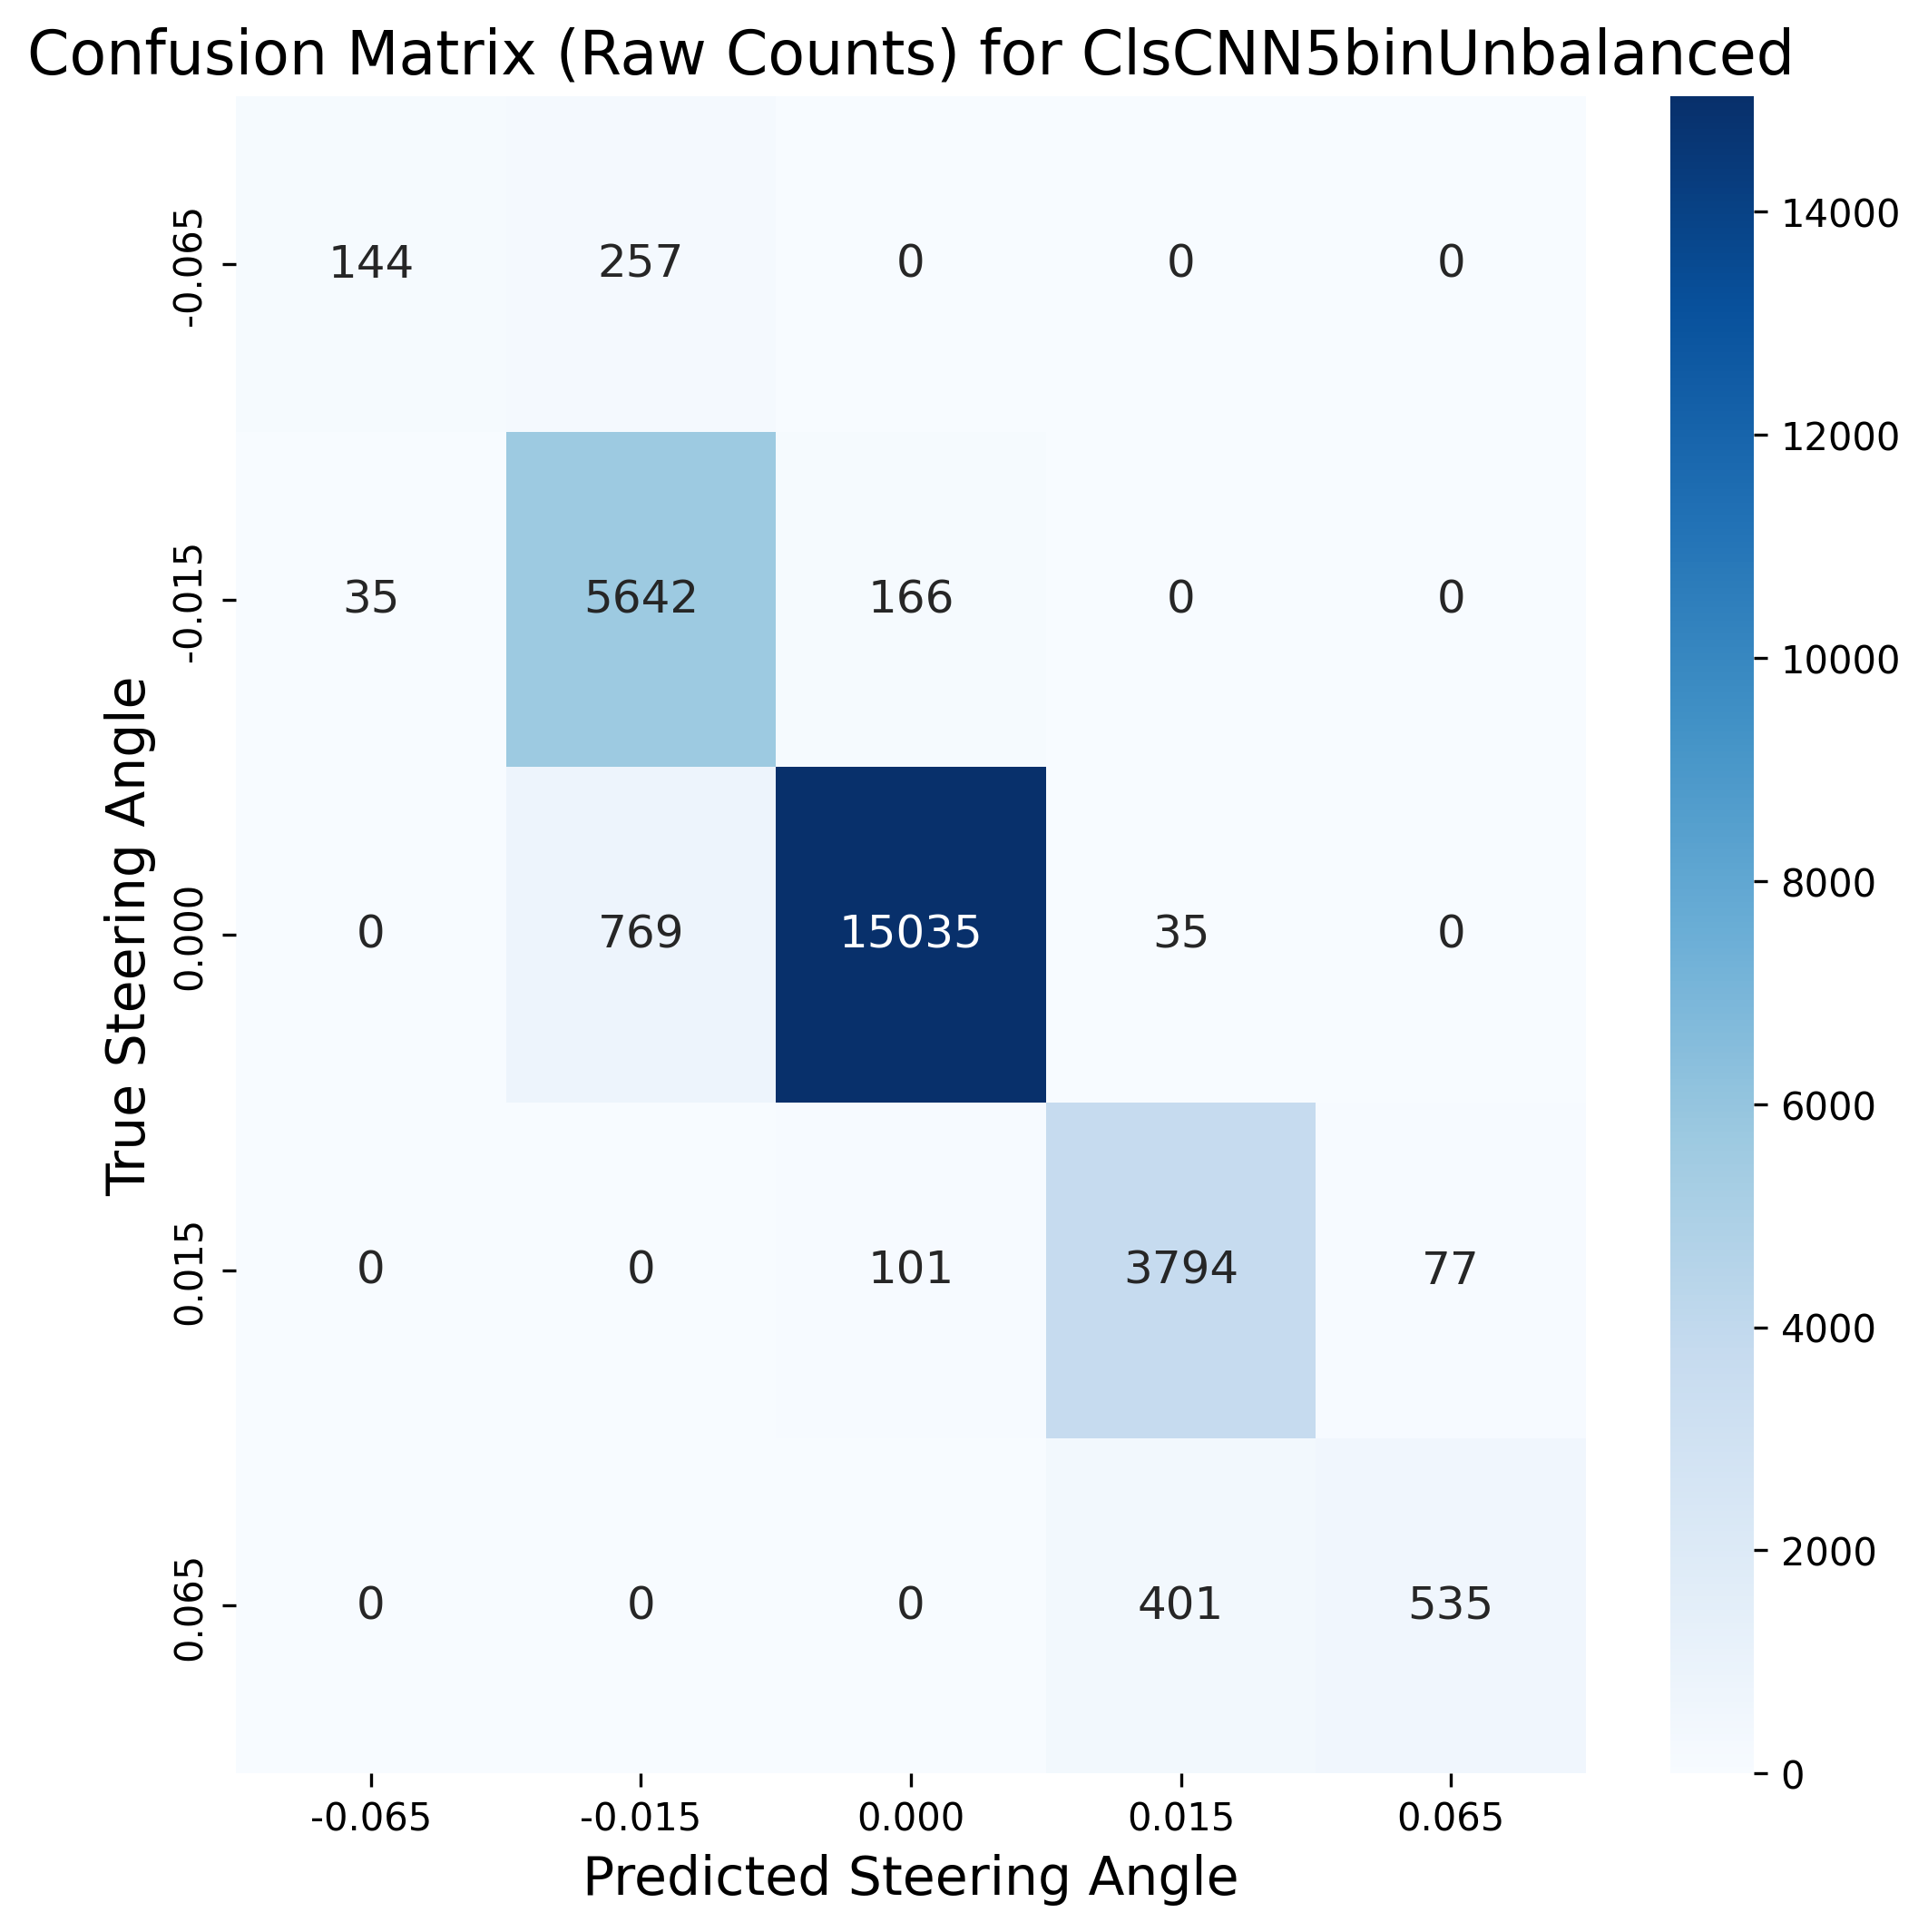
\includegraphics[width=0.65\linewidth]{Figures/Results/cm_raw_ClsCNN5binUnbalanced.png}
\caption{ClsCNN5binUnbalanced model raw counts confusion matrix}
\label{fig:cm_raw_ClsCNN5binUnbalanced}
\end{figure}

\begin{figure}[H]
    \centering
    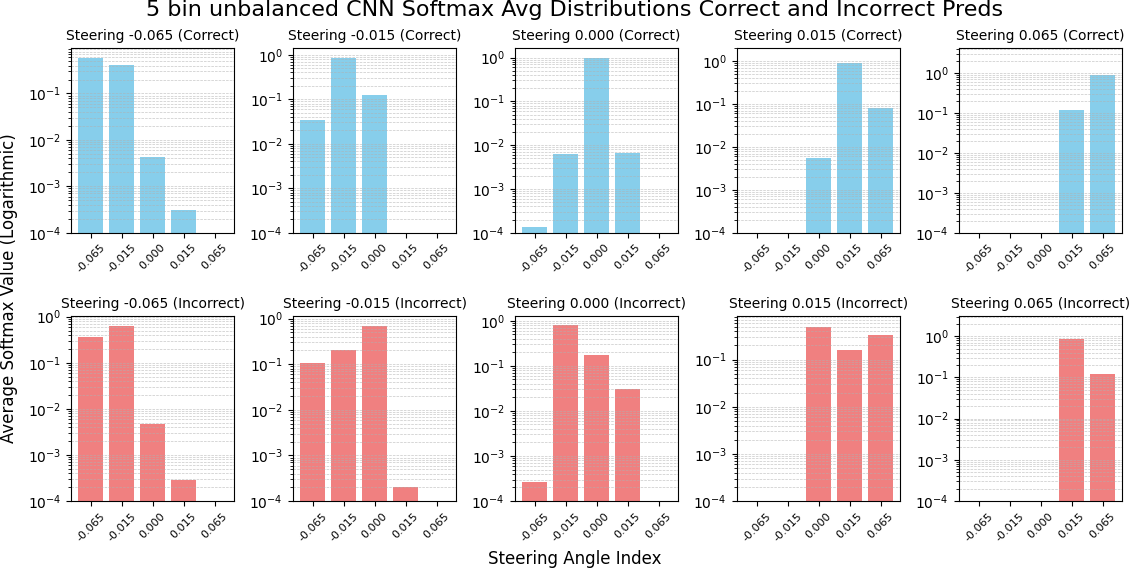
\includegraphics[width=1\linewidth]{Figures/Results/5_bins_cnn_softmax_dist_plot_unbalanced.png}
    \caption{Average softmax Probabilities for Correctly and Incorrectly Classified Steering Angles in the 5 bin cnn unbalanced training Dataset.}
    \label{fig:5_bins_cnn_softmax_dist_unbalanced}
\end{figure}

%%%%%%%%%%%%%%%%%%%%%%
% ClsViT3binBalanced %
%%%%%%%%%%%%%%%%%%%%%%

\textbf{ClsViT3binBalanced}

The ClsViT3binBalanced model was trained using a balanced dataset comprising three discrete steering angle classes corresponding to left, straight, and right maneuvers. Each class contained 22,460 test samples, ensuring uniform class representation during evaluation.

The model achieved an overall classification accuracy of 97.97\% with a mean confidence of 0.9765 across 67,380 test images. Class-wise analysis indicates consistent performance, with precision values between 0.96 and 1.00 and recall values between 0.94 and 1.00. The left and right steering classes ($-0.065$ and $+0.065$) were predicted with near-perfect recall, while the straight class ($0.000$) exhibited a slightly lower recall (0.94), suggesting limited confusion between straight and turning maneuvers.

The macro-averaged precision, recall, and F1-score were each 0.98, confirming balanced performance across classes. These results indicate that the Vision Transformer architecture can effectively capture visual cues relevant to steering direction under a three-bin discretization scheme. The model demonstrates stable behavior in predicting coarse steering categories, supporting its suitability as a perception-based classification component in autonomous driving pipelines.

\begin{table}[htbp]
\centering
\begin{tabular}{@{}lcccc@{}}
\toprule
\textbf{Class} & \textbf{Precision} & \textbf{Recall} & \textbf{F1-Score} & \textbf{Support} \\
\midrule
$-0.065$ & 0.98 & 1.00 & 0.99 & 22,460 \\
$\phantom{-}0.000$ & 1.00 & 0.94 & 0.97 & 22,460 \\
$\phantom{-}0.065$ & 0.96 & 1.00 & 0.98 & 22,460 \\
\midrule
\textbf{Macro Avg} & \textbf{0.98} & \textbf{0.98} & \textbf{0.98} & \textbf{67,380} \\
\bottomrule
\end{tabular}
\caption{Classification performance results for the ClsViT3binBalanced model. The model achieved an overall accuracy of 97.97\% with a mean confidence of 0.9765 across 67,380 test images.}
\label{tab:clf_report_ClsViT3binBalanced}
\end{table}

\begin{figure}[H]
\centering
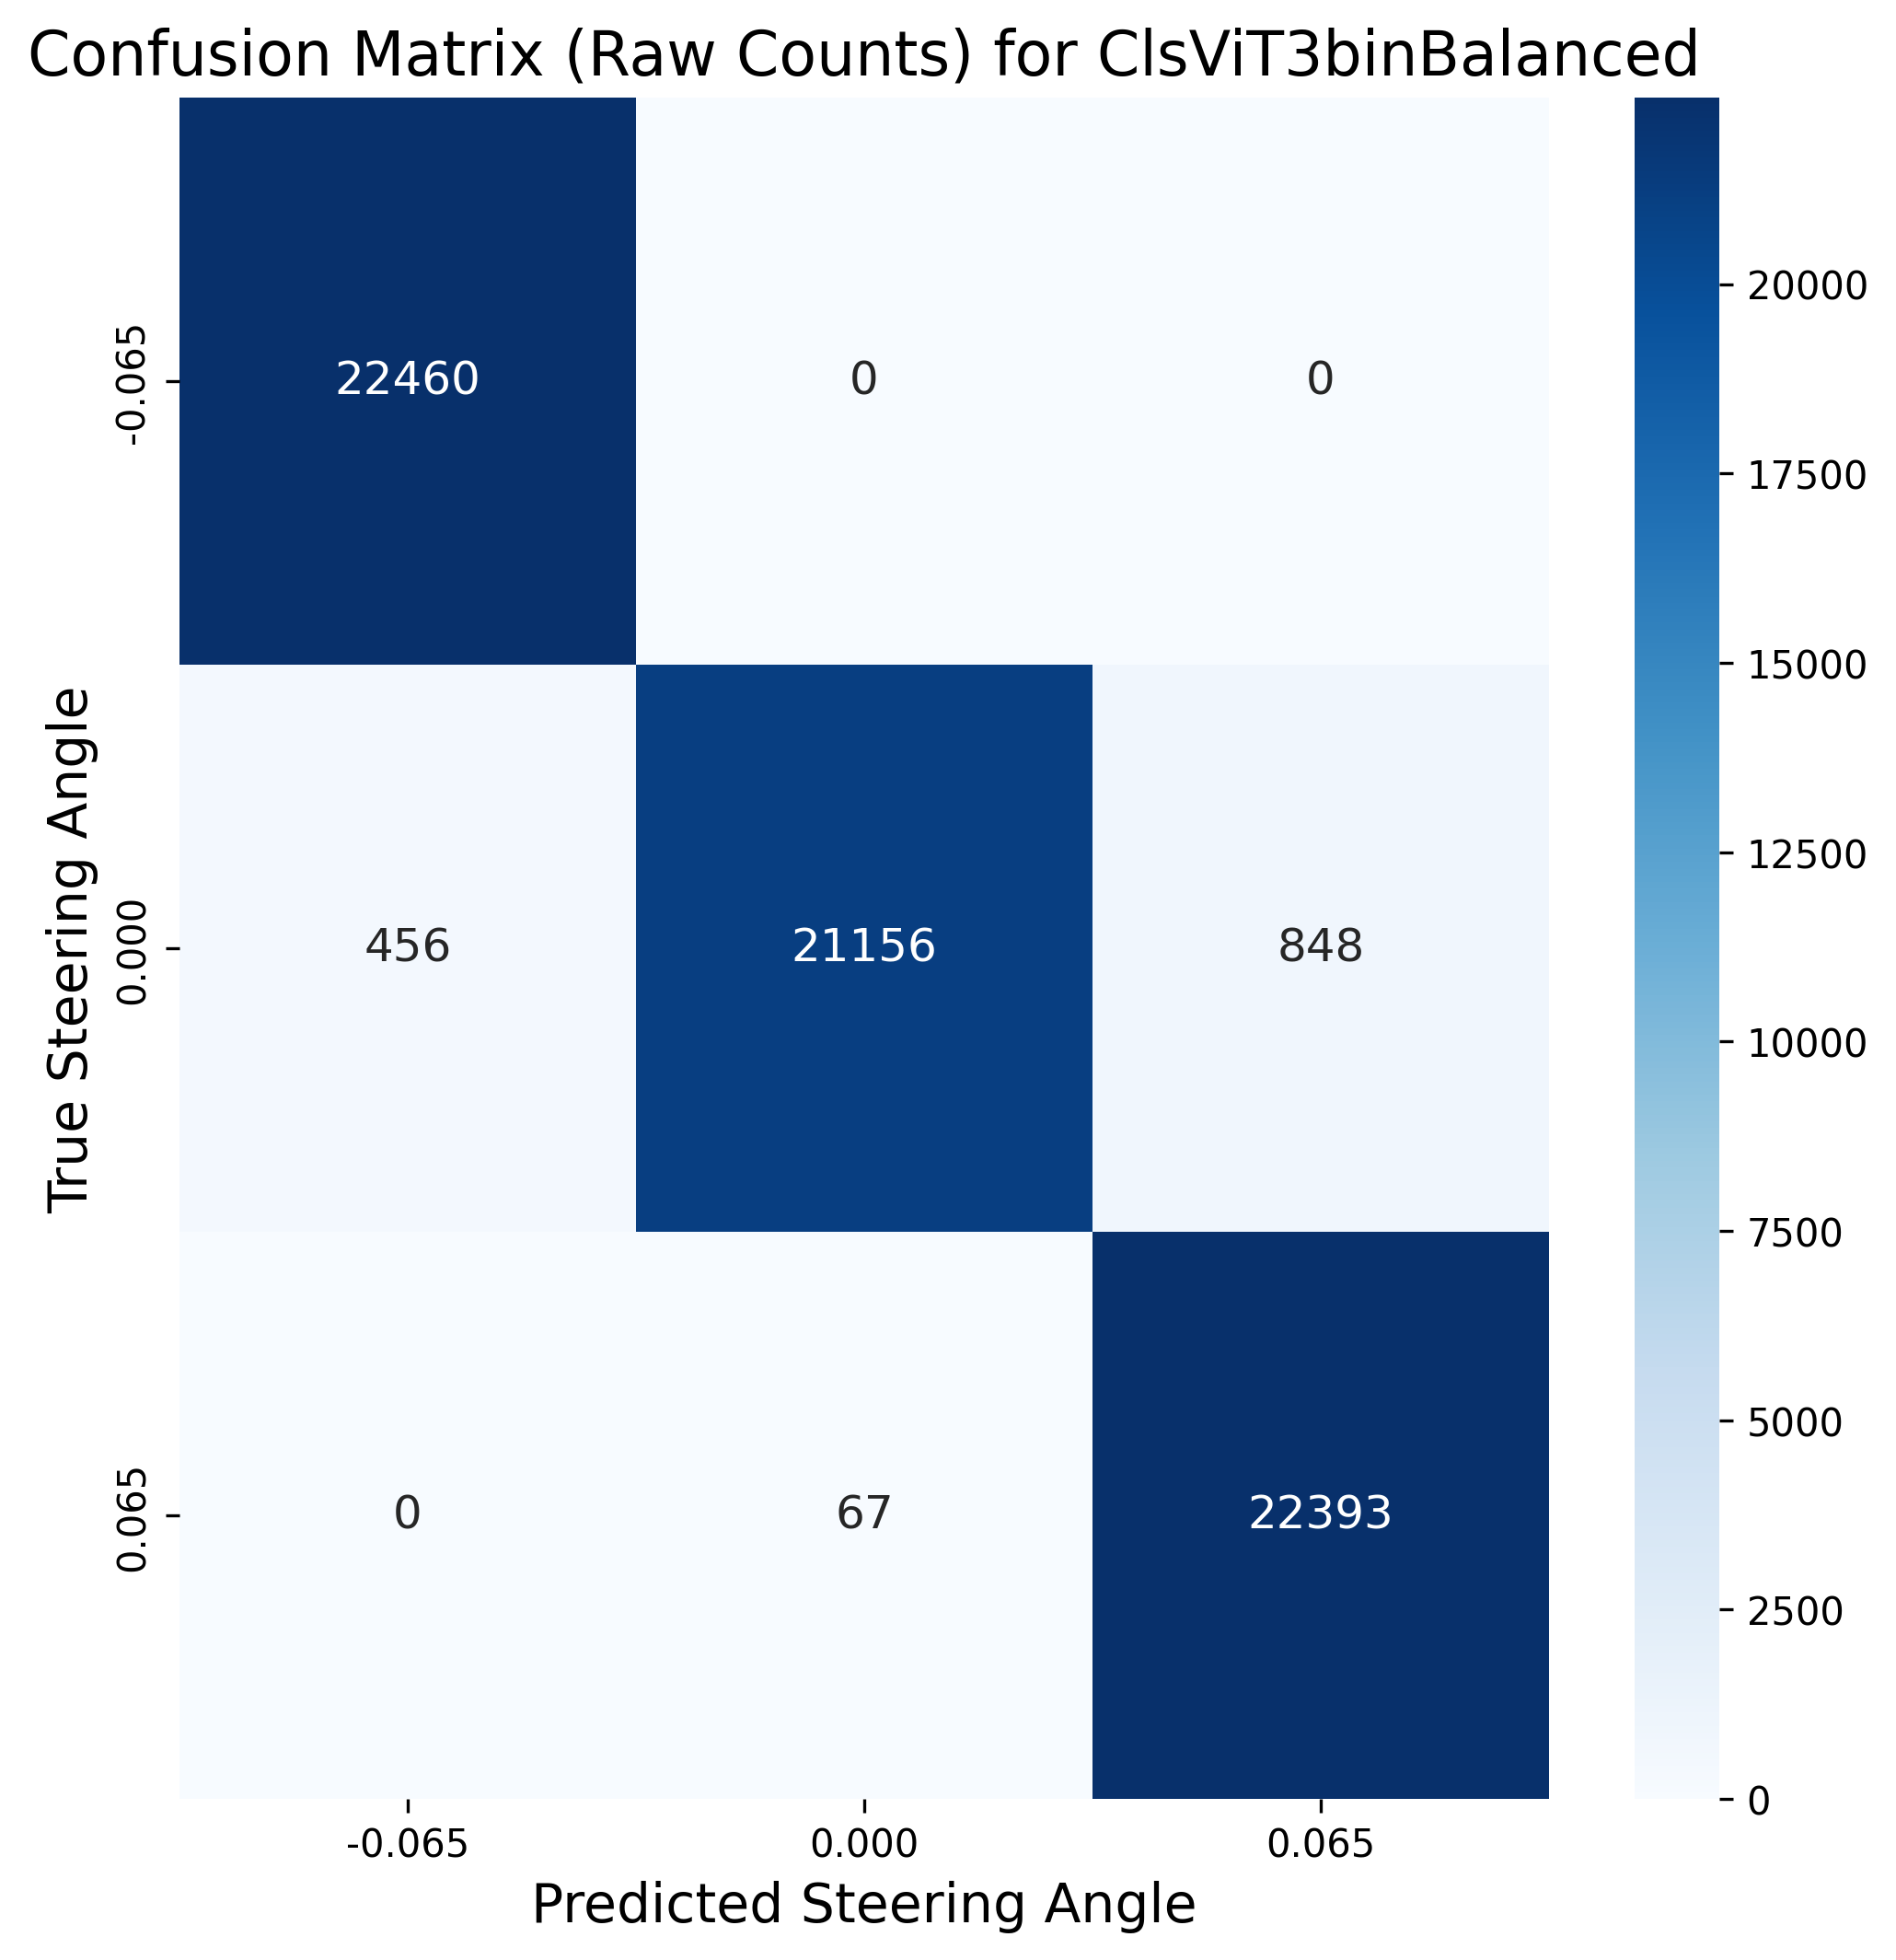
\includegraphics[width=0.65\linewidth]{Figures/Results/cm_raw_ClsViT3binBalanced.png}
\caption{ClsViT3binBalanced model raw counts confusion matrix}
\label{fig:cm_raw_ClsViT3binBalanced}
\end{figure}

\begin{figure}[H]
    \centering
    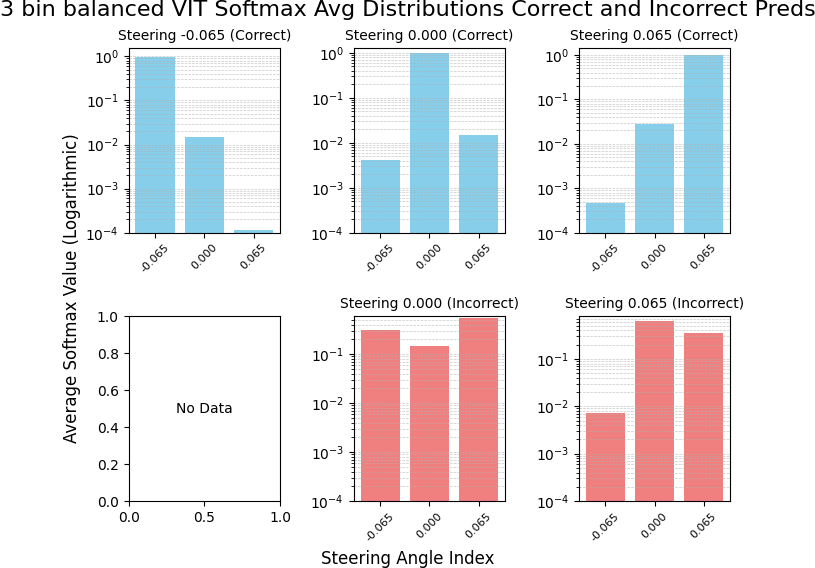
\includegraphics[width=1\linewidth]{Figures/Results/3_bins_vit_softmax_dist_plot_balanced.png}
    \caption{Average softmax Probabilities for Correctly and Incorrectly Classified Steering Angles in the 3 bin vit balanced training Dataset.}
    \label{fig:3_bins_vit_softmax_dist_balanced}
\end{figure}

%%%%%%%%%%%%%%%%%%%%%%
% ClsViT5binBalanced %
%%%%%%%%%%%%%%%%%%%%%%

\textbf{ClsViT5binBalanced}

The ClsViT5binBalanced model was evaluated on a balanced dataset containing five discrete steering angle bins, representing a finer discretization of steering behaviour compared to the three-bin configuration. Each class comprised 15,839 test samples, maintaining equal representation across left, near-left, straight, near-right, and right steering categories.

The model achieved an overall accuracy of 97.77\% with a mean confidence of 0.9779 across 79,195 test images. Performance across all classes was consistent, with precision and recall values ranging between 0.95 and 1.00. The outermost bins ($\pm0.065$) achieved perfect or near-perfect recall, while intermediate bins ($\pm0.015$) and the straight class ($0.000$) showed slightly lower recall (0.95–0.99). These results indicate that the Vision Transformer maintains stable predictive performance even under finer steering quantization, without significant degradation across bins.

The macro-averaged precision, recall, and F1-score were each 0.98, confirming uniform classification performance across all steering directions. Overall, the results demonstrate that the ViT architecture generalizes effectively under balanced training conditions, capturing spatial and contextual dependencies relevant to steering classification in the five-bin discretization framework.

\begin{table}[htbp]
\centering
\begin{tabular}{@{}lcccc@{}}
\toprule
\textbf{Class} & \textbf{Precision} & \textbf{Recall} & \textbf{F1-Score} & \textbf{Support} \\
\midrule
$-0.065$ & 0.99 & 1.00 & 1.00 & 15,839 \\
$-0.015$ & 0.96 & 0.99 & 0.97 & 15,839 \\
$\phantom{-}0.000$ & 0.99 & 0.95 & 0.97 & 15,839 \\
$\phantom{-}0.015$ & 1.00 & 0.95 & 0.97 & 15,839 \\
$\phantom{-}0.065$ & 0.96 & 1.00 & 0.98 & 15,839 \\
\midrule
\textbf{Macro Avg} & \textbf{0.98} & \textbf{0.98} & \textbf{0.98} & \textbf{79,195} \\
\bottomrule
\end{tabular}
\caption{Classification performance results for the ClsViT5binBalanced model. The model achieved an overall accuracy of 97.77\% with a mean confidence of 0.9779 across 79,195 test images.}
\label{tab:clf_report_ClsViT5binBalanced}
\end{table}

\begin{figure}[H]
\centering
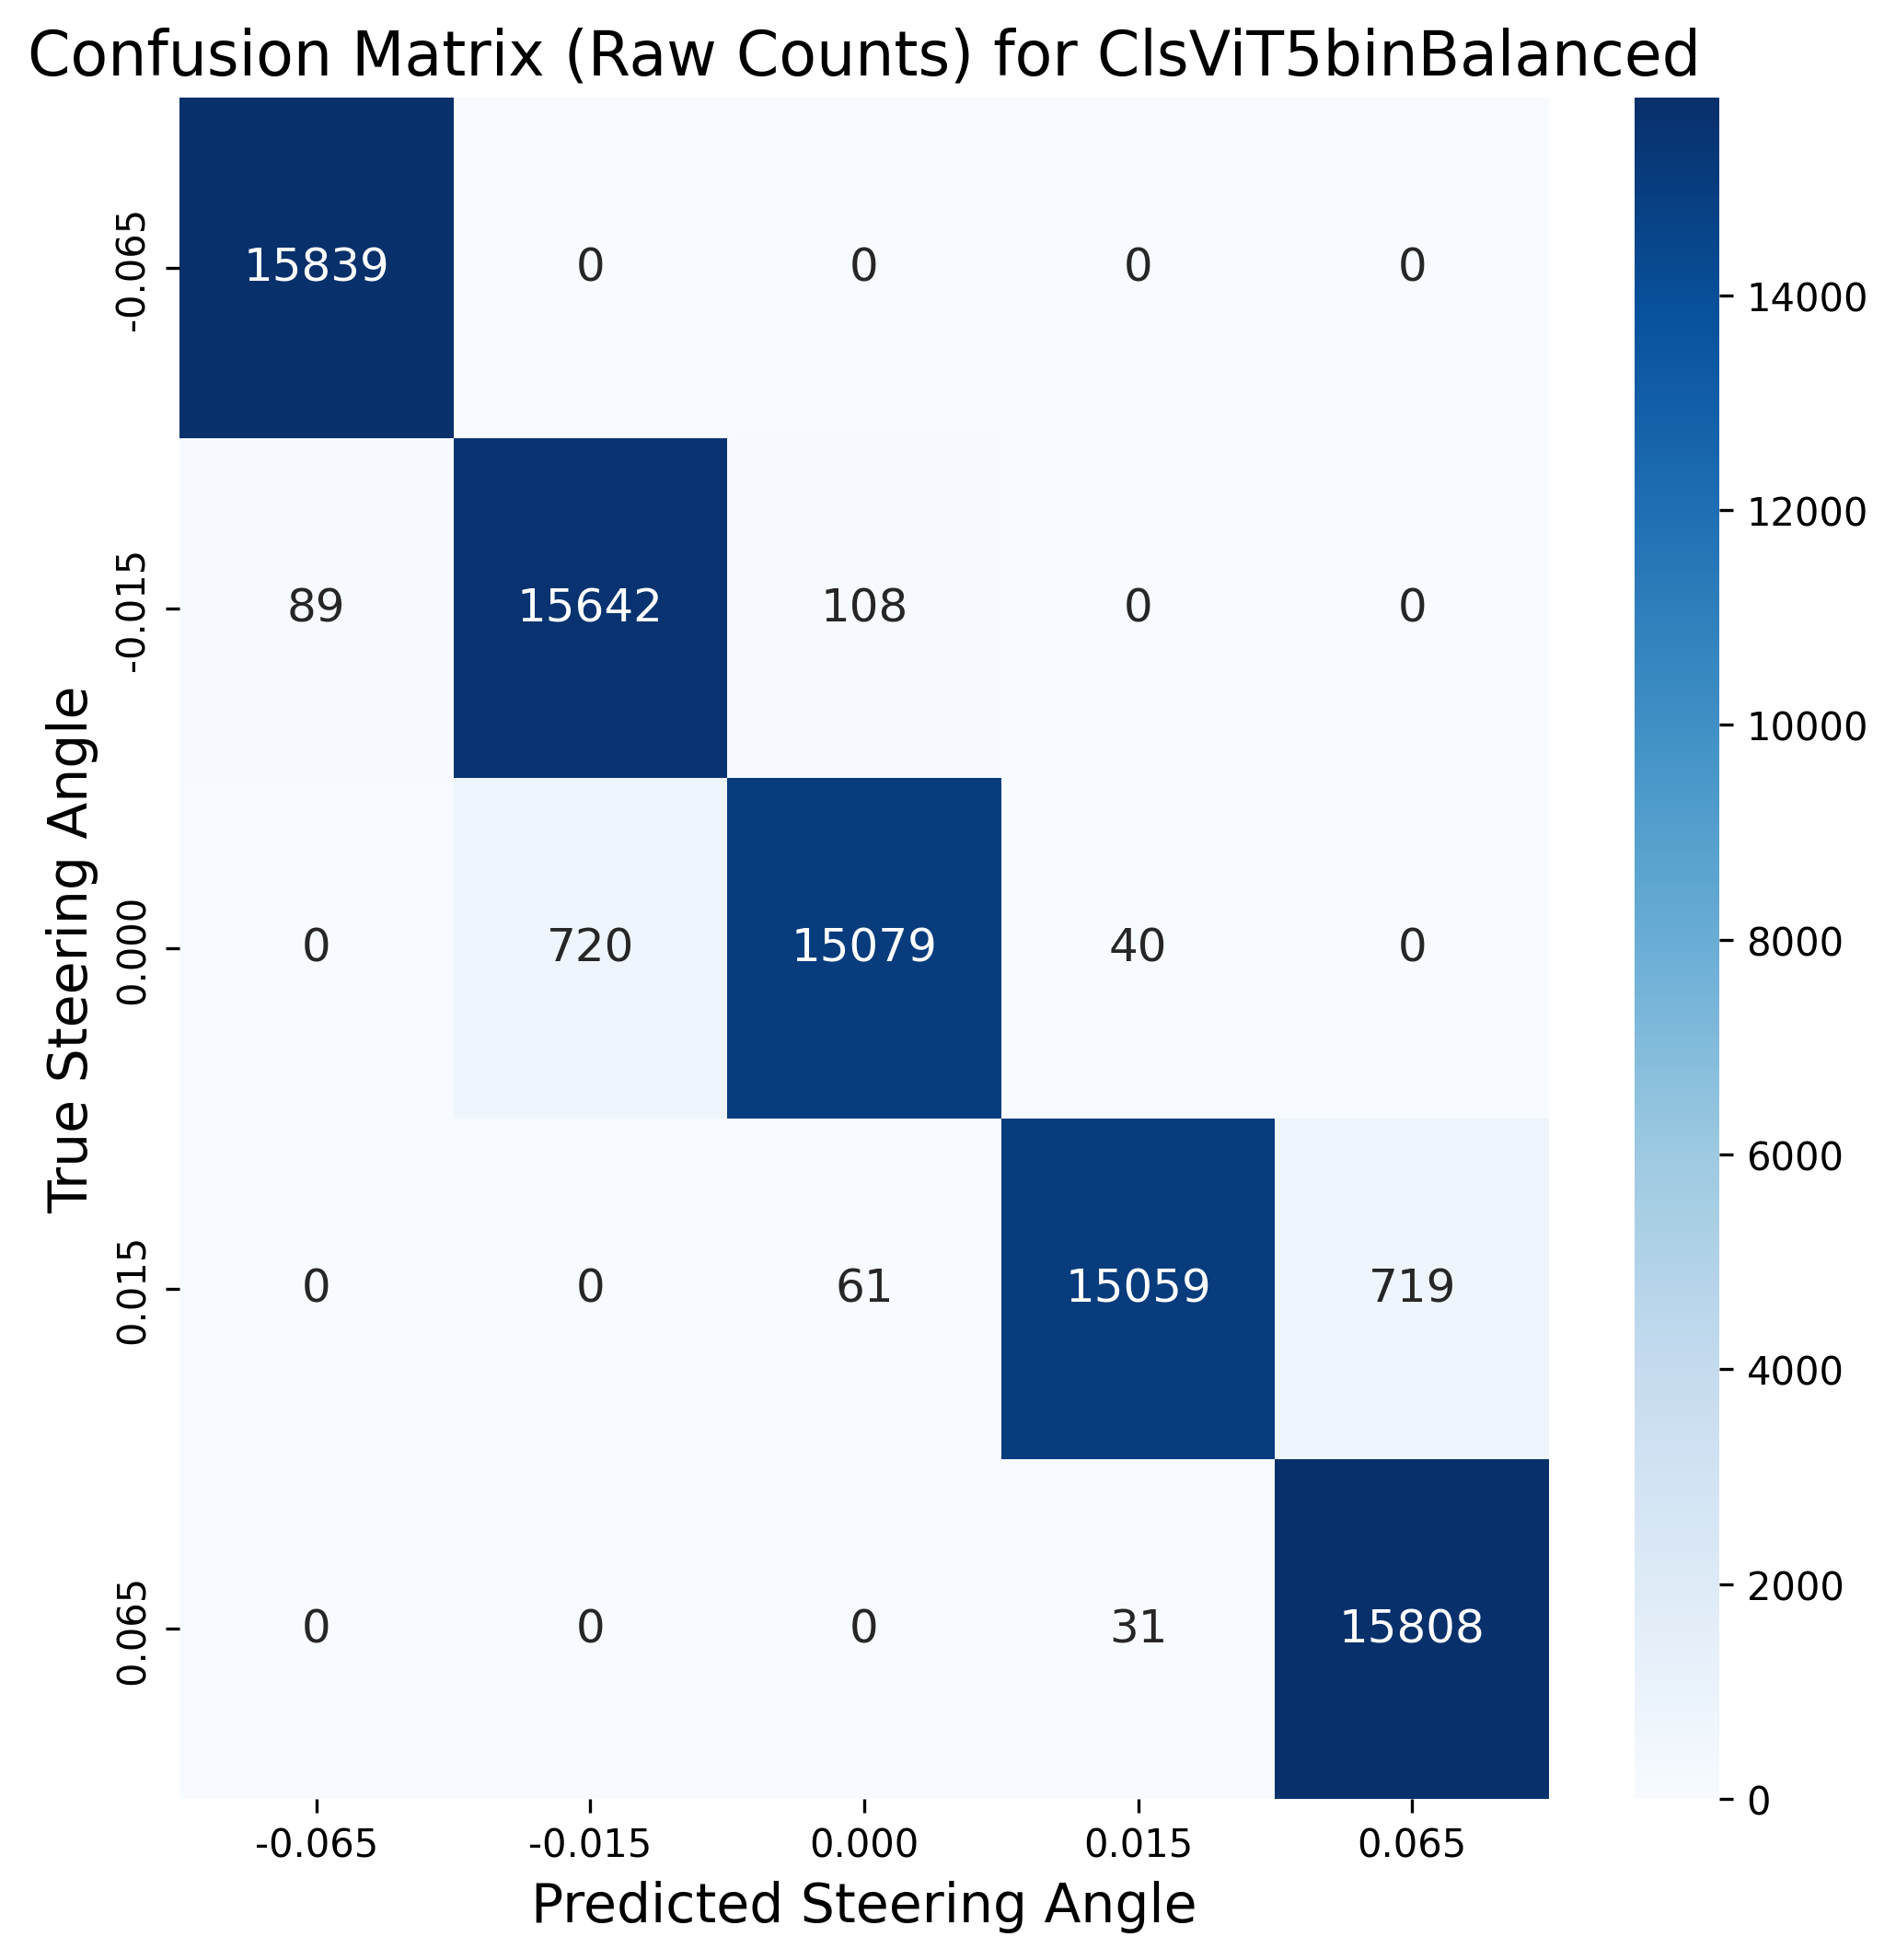
\includegraphics[width=0.65\linewidth]{Figures/Results/cm_raw_ClsViT5binBalanced.png}
\caption{ClsViT5binBalanced model raw counts confusion matrix}
\label{fig:cm_raw_ClsViT5binBalanced}
\end{figure}

\begin{figure}[H]
    \centering
    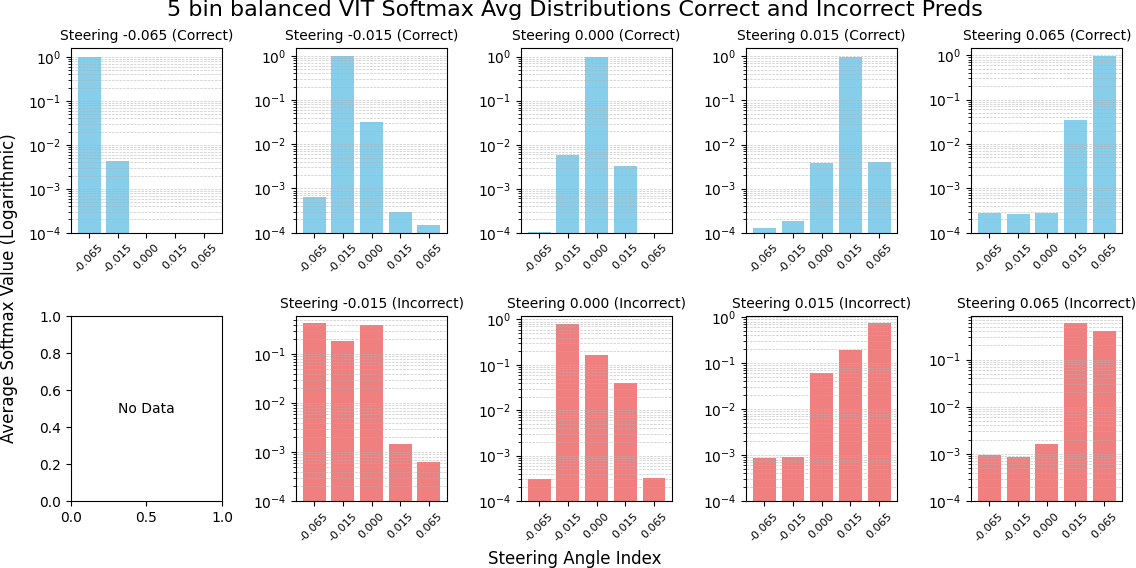
\includegraphics[width=1\linewidth]{Figures/Results/5_bins_vit_softmax_dist_plot_balanced.png}
    \caption{Average softmax Probabilities for Correctly and Incorrectly Classified Steering Angles in the 5 bin vit balanced training Dataset.}
    \label{fig:5_bins_vit_softmax_dist_balanced}
\end{figure}

%%%%%%%%%%%%%%%%%%%%%%%%%%%%%%%%%%%%%%
% NOISE IN SELF-DRIVING APPLICATIONS %
%%%%%%%%%%%%%%%%%%%%%%%%%%%%%%%%%%%%%%

\section{Classifier Models in Self-Driving Applications}

Channel-wise salt-and-pepper noise is applied to the RGB image by first calculating the noise probability $p = \text{intensity} \times 0.01$, then generating a three-dimensional boolean mask $M$ with the same shape as the RGB image where each element $M_{i,j,k}$ (for pixel $(i,j)$ and colour channel $k \in \{R,G,B\}$) is set to True with probability $p$. The mask is then applied to a copy of the original RGB image where each True element in the mask corresponds to a colour channel that gets corrupted: the original channel value $I_{i,j,k}$ is replaced with a new value $I'_{i,j,k} = \text{random}(0,1) \times 255$, which results in either 0 or 255. Since each of the three RGB channels is independently corrupted, a single pixel can exhibit any of the eight possible colour combinations shown in Table \ref{tab:channel_wise_salt_pepper_colors}, ranging from pure black (when all channels are set to 0) to pure white (when all channels are set to 255), with intermediate colours like red, green, blue, cyan, magenta, and yellow when channels are mixed.

\begin{longtable}{@{}llll@{}}
\toprule
R & G & B & Resulting Colour \\
\midrule
\endfirsthead
\toprule
R & G & B & Resulting Colour \\
\midrule
\endhead
0 & 0 & 0 & Black \\
0 & 0 & 255 & Blue \\
0 & 255 & 0 & Green \\
0 & 255 & 255 & Cyan \\
255 & 0 & 0 & Red \\
255 & 0 & 255 & Magenta \\
255 & 255 & 0 & Yellow \\
255 & 255 & 255 & White \\
\bottomrule
\caption{Possible pixel values and colours when channel-wise salt-and-pepper noise is applied independently to RGB channels}
\label{tab:channel_wise_salt_pepper_colors}
\end{longtable}




%%%%%%%%%%%%%%%%%%%%%%%%%%%%%%%%%%%%%%%%%%%%%%%%%%%
% FIGURE - COMBINED 3%, 10%, 50% NOISE APPLIED TO %
% VEHICLE CAMERA                                  %
%%%%%%%%%%%%%%%%%%%%%%%%%%%%%%%%%%%%%%%%%%%%%%%%%%%

\begin{figure}[H]
    \centering
    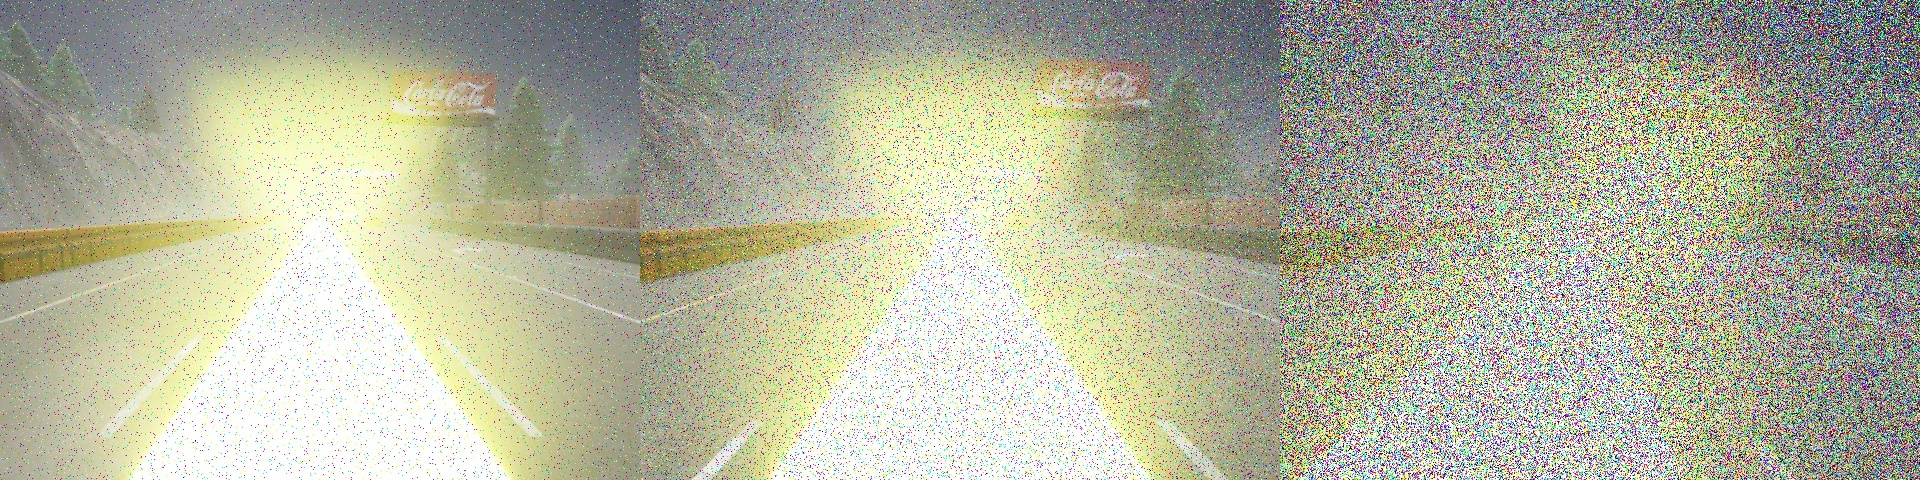
\includegraphics[width=1.0\linewidth]{Figures/Results/experiment-247-251-255-3pc-10pc-50pc-rbg-pepper-noise-combined.jpg}
    \caption{CARLA simulator vehicle camera RGB image with 3\% (left), 10\% (middle) and 50\% channel-wise salt-and-pepper noise applied}
    \label{fig:experiment-247-251-255-3pc-10pc-50pc-rbg-pepper-noise-combined}
\end{figure}

Figure \ref{fig:experiment-247-251-255-3pc-10pc-50pc-rbg-pepper-noise-combined} shows images as would be presented to CNN (before preprocessing) and ViT networks (as is) for steering prediction. The image is generated by starting the simulation and saving one image. The images with channel-wise salt-and-pepper noise shown in the figure, were generated from left to right by experiments 247, 251 and 255.

\textbf{Self-driving softmax Output Analysis}

%%%%%%%%%%%%%%%%%%%%%%%%%%%%%%%%%%%%%%%%%%%%
% FIGURES NOISE METRICS WITH LANE INVASION %
%%%%%%%%%%%%%%%%%%%%%%%%%%%%%%%%%%%%%%%%%%%%


% figures generated by experiment 268




%%%%%%%%%%%%%%%%%%%%%%%%%%%%%%%%%%%%%%%%%%%%%%
% COMBINED DISTANCE METRICS - EXPERIMENT 268 %
%%%%%%%%%%%%%%%%%%%%%%%%%%%%%%%%%%%%%%%%%%%%%%

% NB Experiment 268 aggregates values from 
\begin{figure}[H]
    \centering
    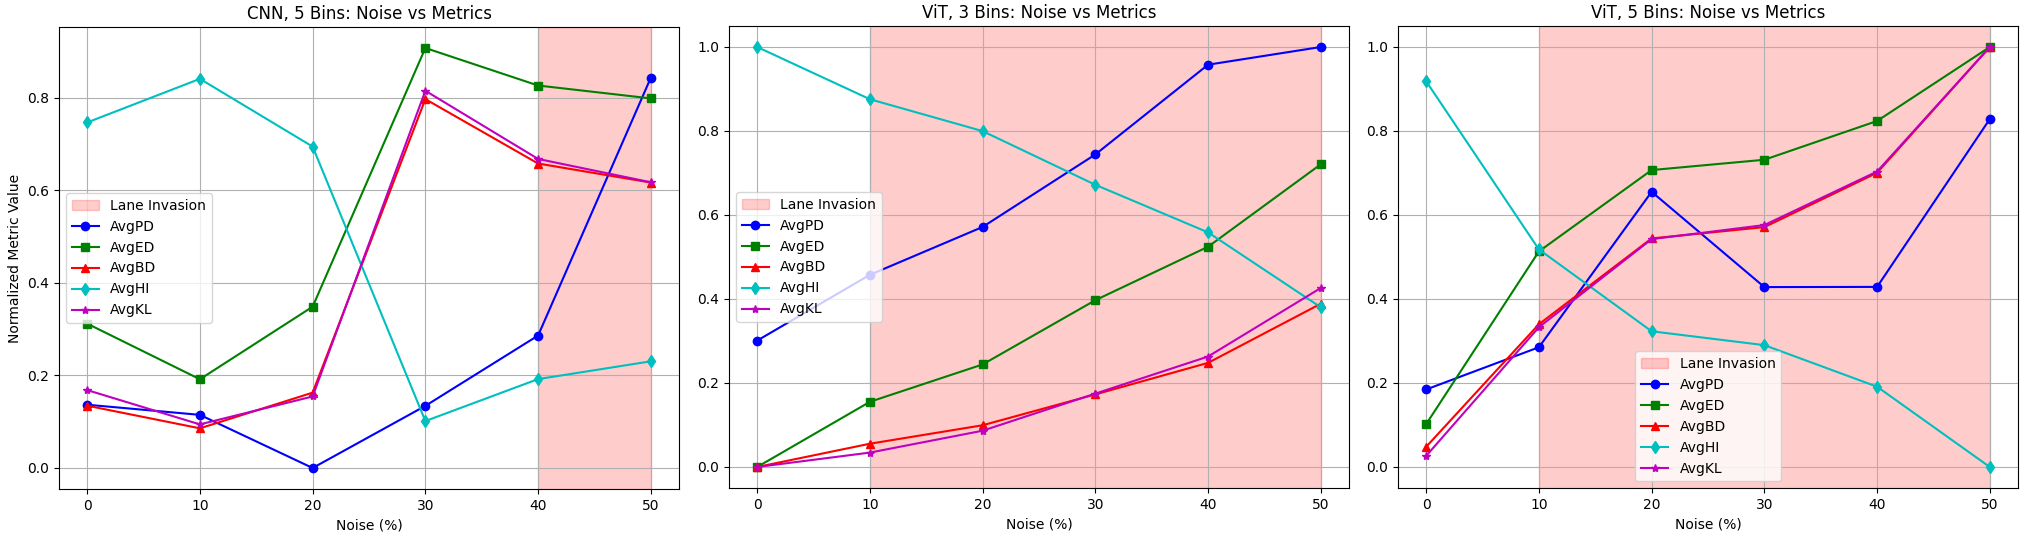
\includegraphics[width=1.0\linewidth]{Figures/Results/combined_cnn_5bin_vit_3bin_vit_5bin_noise_distance_metrics.png}
    \caption{Combined CNN 5 bin (left), ViT 3 bin (middle) and ViT 5 bin (right) noise levels by Average Path Distance (blue), Average Euclidean Distance (green), Average Bhattacharyya Distance (red), Average Histogram Intersection (cyan) and Average KL Divergence (purple). The pink band indicates noise levels where lane invasions occurred}
    \label{fig:combined_cnn_5bin_vit_3bin_vit_5bin_noise_distance_metrics}
\end{figure}

Figure \ref{fig:combined_cnn_5bin_vit_3bin_vit_5bin_noise_distance_metrics}, shows the general trend that as noise levels increase, all distance metrics also increase, except Histogram Intersection, which has a maximum value of 1 when images all RGB pixels are identical (0\% noise), and decreases as noise is added, original and noisy image becoming dissimilar.
To obtain one data point in the plot, pepper noise is applied to the RGB image at 0, 10, 20, 30, 40 and 50\% pixel ratios. An average is taken for all predicted softmax output Euclidean distances to centroids, across all classes (AvgED). An average distance is taken from the vehicle to the lane path across all path distance readings acquired during the simulation (AvgPD). The following averages are taken between the original image and the noisy image for all images generated by the simulation: Bhattacharyya Distance (AvgBD), Histogram Intersection (AvgHI), KL Divergence (AvgKL). Min-max normalization was applied to the averages being plotted, following the formula $x_{norm} = (x - x_{min}) / (x_{max} - x_{min})$, which scales all values to the range [0,1].

Bhattacharyya Distance, Histogram Intersection and KL Divergence cannot be quantified in real world conditions because, unlike simulated scenarios, there is no "reference" image to be compared with. The metrics are still useful to confirm there exists a level of separation between the captured image and the image presented to the network, given noise. Distance to path cannot be quantified in real world conditions because the simulated path is determined by objects (waypoints) generated by the simulation, which exist as transform objects in simulation but not in the real world. The key metric, determining if the model is "outside of its comfort zone", is the Average Euclidean Distance. The Euclidean distance between the network's softmax output and the pre-computed class (discretized steering angles) centroids is the only quantity that can be computed in the wild.
The pink region of the plots mark the occurrence of lane invasions. For example, the left hand side plot for the CNN trained on 5 bin quantized (-0.065, -0.015, 0.0000, 0.0150 and 0.0650 steering angle classes) balanced data: , presented lane invasions where at 40\% noise, where 40\% noise would approximately correspond to the right hand side image in Figure \ref{fig:combined_cnn_5bin_vit_3bin_vit_5bin_noise_distance_metrics}. 

Table \ref{tab:experiment_stats_common_0_10_20_30_40_50} presents results for experiments that were common to the three models tested - the best performing CNN model (5 bin-quantized unbalanced-dataset, 93.18\% overall accuracy) the corresponding best performing 5 bin-quantized balanced-dataset ViT model (97.77\% overall accuracy) and the best performing model overall, the ViT 3 bin-quantized balanced-dataset model (97.97\% overall accuracy).

Further, Table \ref{tab:experiment_stats_common_0_10_20_30_40_50} presents the original values used to compute the plots in Figure \ref{fig:combined_cnn_5bin_vit_3bin_vit_5bin_noise_distance_metrics}. The bold font in consecutive rows, column AvgED, shows where a lane invasion was observed. For example, in experiment 240, the CNN 5 bin model steering, with front facing camera images subject to 40\% noise, lead to a lane invasion (column LI presenting value T). The lane invasion lead to the simulation being stopped at frame count 10133 (FrCnt). The average distance to the optimal trajectory path (AvrPD) was recorded at 0.1080 units of distance for the all distance to path readings (PDCont), the average Euclidean distance to predicted class centroid (AvgED) was recorded at 0.6257 (across all predictions, corresponding in number to the frame count FrCnt). In general the average Bhattacharya Distance (AvgBD) and KL Divergence (AvgKL) tend to increase with noise, while Histogram Intersection (AvgHI) tends to decrease with noise.
The average Euclidean distance to the predicted class centroid (AvgED) tend to increase with noise. 
Since the aim is to ensure autonomous system safety, a prediction, under the experimental parameters, can be considered safe when no lane invasion occurs. Therefore, we make note of the nearest average Euclidean distance to predicted class centroid, where a lane invasion occurred while the simulated vehicle was steering with predictions from the CNN 5 bin classifier. The nearest average (lowest value) was observed in experiment 241, 0.6061. We note that there are higher averages - experiment 239, 30\% noise, 0.6828 - where lane invasions did not occur. Our choice for threshold for the CNN 5 bin model should be between 0.6061 and 0.2829 average Euclidean distance from the class softmax outputs to the predicted class centroids. In other words, the threshold should be placed between the highest AvgED value where a lane invasion did not occur and the lowest AvgED value where a lane invasion occurred, for a given model. We highlight the values in boldface in Table \ref{tab:experiment_stats_common_0_10_20_30_40_50}. In short, for the CNN 5 bin classifier, the threshold should be placed between 0.2892 and 0.6061. 

Based on the common results, for noise levels 0, 10, 20, 30, 40 and 50\%, and applying the same constraints, the ViT 3 bin threshold should be placed between 0.0437 and 0.1530. In practice, the ViT 3 bin model presented lane invasions at lower noise levels compared to the CNN 5 bin model, leading to shorter intervals. 
We present the full results in Table \ref{tab:experiment_stats}.

%%%%%%%%%%%%%%%%%%%%%%%%%%%%%%%%%%%%%%%%%%%%%%%%%%%%
% COMMON RESULTS TABLE (0,10,20,30,40,50pct noise) %
%%%%%%%%%%%%%%%%%%%%%%%%%%%%%%%%%%%%%%%%%%%%%%%%%%%%

\begin{longtable}{@{}cllrrrrrrrrrc@{}}
\toprule
Exp & Net & Bins & Noise & AvgPD & PDCnt & AvgED & AvgBD & AvgHI & AvgKL & FrCnt & LI \\
\midrule
\endfirsthead
\toprule
Exp & Net & Bins & Noise & AvgPD & PDCnt & AvgED & AvgBD & AvgHI & AvgKL & FrCnt & LI \\
\midrule
\endhead
262 & CNN & 5 & 0 & 0.0600 & 1032 & 0.2634 & 0.0706 & 0.8091 & 0.1016 & 19749 & F \\
237 & CNN & 5 & 10 & 0.0529 & 1032 & 0.1787 & 0.0493 & 0.8681 & 0.0699 & 20534 & F \\
238 & CNN & 5 & 20 & 0.0160 & 1032 & \textbf{0.2892} & 0.0829 & 0.7765 & 0.0957 & 22356 & F \\
239 & CNN & 5 & 30 & 0.0592 & 1032 & 0.6828 & 0.3588 & 0.4053 & 0.3785 & 22375 & F \\
240 & CNN & 5 & 40 & 0.1080 & 473 & 0.6257 & 0.2982 & 0.4621 & 0.3154 & 10133 & T \\
241 & CNN & 5 & 50 & 0.2871 & 473 & \textbf{0.6061} & 0.2803 & 0.4861 & 0.2938 & 10550 & T \\
263 & ViT & 3 & 0 & 0.1127 & 1032 & \textbf{0.0437} & 0.0120 & 0.9676 & 0.0296 & 8736 & F \\
251 & ViT & 3 & 10 & 0.1631 & 17 & \textbf{0.1530} & 0.0362 & 0.8898 & 0.0443 & 130 & T \\
252 & ViT & 3 & 20 & 0.1997 & 15 & 0.2156 & 0.0553 & 0.8423 & 0.0666 & 108 & T \\
253 & ViT & 3 & 30 & 0.2552 & 12 & 0.3234 & 0.0872 & 0.7623 & 0.1044 & 90 & T \\
254 & ViT & 3 & 40 & 0.3238 & 8 & 0.4130 & 0.1199 & 0.6914 & 0.1422 & 58 & T \\
255 & ViT & 3 & 50 & 0.3374 & 5 & 0.5513 & 0.1811 & 0.5798 & 0.2120 & 34 & T \\
266 & ViT & 5 & 0 & 0.0753 & 1032 & \textbf{0.1156} & 0.0330 & 0.9165 & 0.0409 & 4358 & F \\
256 & ViT & 5 & 10 & 0.1076 & 39 & \textbf{0.4051} & 0.1599 & 0.6660 & 0.1720 & 164 & T \\
257 & ViT & 5 & 20 & 0.2266 & 25 & 0.5415 & 0.2488 & 0.5440 & 0.2618 & 101 & T \\
258 & ViT & 5 & 30 & 0.1537 & 30 & 0.5588 & 0.2605 & 0.5234 & 0.2761 & 120 & T \\
259 & ViT & 5 & 40 & 0.1538 & 40 & 0.6238 & 0.3167 & 0.4615 & 0.3307 & 157 & T \\
260 & ViT & 5 & 50 & 0.2823 & 29 & 0.7479 & 0.4470 & 0.3418 & 0.4576 & 114 & T \\
\bottomrule
\caption{Common experiment results for noise levels 0\%, 10\%, 20\%, 30\%, 40\%, and 50\% across three models: CNN 5-bin (unbalanced dataset, 93.18\% accuracy), ViT 5-bin (balanced dataset, 97.77\% accuracy), and ViT 3-bin (balanced dataset, 97.97\% accuracy). The table reports metrics including average path deviation (AvgPD), path deviation count (PDCnt) - this is the number of times in the simulation the distance from the vehicle from the path was computed, average Euclidean distance to predicted class centroid (AvgED, bolded where lane invasions occurred), average Bhattacharyya distance (AvgBD), average histogram intersection (AvgHI), average KL divergence (AvgKL), frame count (FrCnt), and lane invasion status (LI, T for true, F for false). These metrics underpin the plots in Figure~\ref{fig:combined_cnn_5bin_vit_3bin_vit_5bin_noise_distance_metrics}. For safety, thresholds for AvgED are proposed to avoid lane invasions: for CNN 5-bin, between 0.2892 (highest safe) and 0.6061 (lowest unsafe); for ViT 3-bin, between 0.0437 and 0.1530; for ViT 5-bin, between 0.1156 and 0.4051.}
\label{tab:experiment_stats_common_0_10_20_30_40_50}
\end{longtable}

% Removed, cannot find this table
% Full results are in Appendix~\ref{AppendixG-full-results}, Table~\ref{tab:experiment_stats_full_0_10_20_30_40_50}.}

% LOD Paper Integration - Theoretical Foundation for Threshold-Based Safety
\textbf{Setting Distance-to-Centroid Thresholds}

The threshold selection methodology for preventing lane invasions applies framework described in the contributions, which demonstrates that Euclidean distance between softmax outputs and class centroids serves as a proxy for prediction confidence. The work establishes that setting distance thresholds based on distances from incorrect predictions to class centroids enables systems to identify unreliable predictions and defer judgment.

In our autonomous driving implementation, this translates to safety thresholds: when steering predictions exceed the distance threshold to their class centroid, the system should reject the prediction as potentially unsafe. The threshold ranges in Table \ref{tab:experiment_stats_common_0_10_20_30_40_50} represent conservative boundaries derived from the minimum distance observed for lane invasions in our simulated scenarios. 

%%%%%%%%%%%%%%%%%%%%%%
% MAIN RESULTS TABLE %
%%%%%%%%%%%%%%%%%%%%%%

% The main thing shown here is that for ViT models lane invasions start with **minimal**
% noise. That can also be stated in the condensed table (to match noise levels for all
% models).

% NOTE: Full results table commented out - move to appendix if needed
% \begin{longtable}{@{}cllrrrrrrrrrc@{}}
% \toprule
% Exp & Net & Bins & Noise & AvgPD & PDCnt & AvgED & AvgBD & AvgHI & AvgKL & FrCnt & LI \\
% \midrule
% \endfirsthead
% \toprule
% Exp & Net & Bins & Noise & AvgPD & PDCnt & AvgED & AvgBD & AvgHI & AvgKL & FrCnt & LI \\
% \midrule
% \endhead
% 262 & CNN & 5 & 0 & 0.0600 & 1032 & 0.2634 & 0.0706 & 0.8091 & 0.1016 & 19749 & F \\
% 237 & CNN & 5 & 10 & 0.0529 & 1032 & 0.1787 & 0.0493 & 0.8681 & 0.0699 & 20534 & F \\
% 238 & CNN & 5 & 20 & 0.0160 & 1032 & 0.2892 & 0.0829 & 0.7765 & 0.0957 & 22356 & F \\
% 239 & CNN & 5 & 30 & 0.0592 & 1032 & 0.6828 & 0.3588 & 0.4053 & 0.3785 & 22375 & F \\
% 240 & CNN & 5 & 40 & 0.1080 & 473 & 0.6257 & 0.2982 & 0.4621 & 0.3154 & 10133 & T \\
% 241 & CNN & 5 & 50 & 0.2871 & 473 & 0.6061 & 0.2803 & 0.4861 & 0.2938 & 10550 & T \\
% 242 & CNN & 5 & 55 & 0.3853 & 189 & 0.5933 & 0.2715 & 0.5011 & 0.2823 & 4146 & T \\
% 243 & CNN & 5 & 60 & 0.3105 & 18 & 0.5292 & 0.2141 & 0.5533 & 0.2342 & 369 & T \\
% 263 & ViT & 3 & 0 & 0.1127 & 1032 & 0.0437 & 0.0120 & 0.9676 & 0.0296 & 8736 & F \\
% 245 & ViT & 3 & 1 & 0.1805 & 217 & 0.1063 & 0.0255 & 0.9232 & 0.0339 & 930 & T \\
% 246 & ViT & 3 & 2 & 0.1163 & 34 & 0.0601 & 0.0148 & 0.9545 & 0.0204 & 144 & T \\
% 247 & ViT & 3 & 3 & 0.1087 & 34 & 0.0617 & 0.0141 & 0.9537 & 0.0184 & 145 & T \\
% 248 & ViT & 3 & 4 & 0.1215 & 34 & 0.0666 & 0.0140 & 0.9507 & 0.0183 & 144 & T \\
% 249 & ViT & 3 & 5 & 0.1360 & 33 & 0.0697 & 0.0149 & 0.9488 & 0.0191 & 140 & T \\
% 250 & ViT & 3 & 7 & 0.1276 & 34 & 0.0727 & 0.0145 & 0.9471 & 0.0185 & 271 & T \\
% 251 & ViT & 3 & 10 & 0.1631 & 17 & 0.1530 & 0.0362 & 0.8898 & 0.0443 & 130 & T \\
% 252 & ViT & 3 & 20 & 0.1997 & 15 & 0.2156 & 0.0553 & 0.8423 & 0.0666 & 108 & T \\
% 253 & ViT & 3 & 30 & 0.2552 & 12 & 0.3234 & 0.0872 & 0.7623 & 0.1044 & 90 & T \\
% 254 & ViT & 3 & 40 & 0.3238 & 8 & 0.4130 & 0.1199 & 0.6914 & 0.1422 & 58 & T \\
% 255 & ViT & 3 & 50 & 0.3374 & 5 & 0.5513 & 0.1811 & 0.5798 & 0.2120 & 34 & T \\
% 266 & ViT & 5 & 0 & 0.0753 & 1032 & 0.1156 & 0.0330 & 0.9165 & 0.0409 & 4358 & F \\
% 256 & ViT & 5 & 10 & 0.1076 & 39 & 0.4051 & 0.1599 & 0.6660 & 0.1720 & 164 & T \\
% 257 & ViT & 5 & 20 & 0.2266 & 25 & 0.5415 & 0.2488 & 0.5440 & 0.2618 & 101 & T \\
% 258 & ViT & 5 & 30 & 0.1537 & 30 & 0.5588 & 0.2605 & 0.5234 & 0.2761 & 120 & T \\
% 259 & ViT & 5 & 40 & 0.1538 & 40 & 0.6238 & 0.3167 & 0.4615 & 0.3307 & 157 & T \\
% 260 & ViT & 5 & 50 & 0.2823 & 29 & 0.7479 & 0.4470 & 0.3418 & 0.4576 & 114 & T \\
% 261 & ViT & 5 & 60 & 0.3657 & 8 & 0.7627 & 0.4828 & 0.3254 & 0.4818 & 34 & T \\
% \bottomrule
% \caption{Experiment Statistics with Lane Invasion, full results}
% \label{tab:experiment_stats}
% \end{longtable}

Table \ref{tab:youtube_links} presents links to video captures of experiments where lane invasions did and did not occur (column LI showing values T and F respectively). The simulation is generated as described in Section \ref{methods:carla}.

\begin{longtable}{@{}clcrcc@{}}
\toprule
Exp & Net & Bins & Noise & LI & YouTube \\
\midrule
\endfirsthead
\toprule
Exp & Net & Bins & Noise & LI & YouTube \\
\midrule
\endhead
262 & CNN & 5 & 0 & F & \href{https://youtu.be/vhbmxwMlZfk}{Video} \\
237 & CNN & 5 & 10 & F & \href{https://youtu.be/3Zsny4NM_NQ}{Video} \\
%238 & CNN & 5 & 20 & F & \href{https://youtu.be/RaCVAlwBQlQ}{Video} \\
239 & CNN & 5 & 30 & F & \href{https://youtu.be/CzJlbYX0CnQ}{Video} \\
240 & CNN & 5 & 40 & T & \href{https://youtu.be/FVlpiNw26J8}{Video} \\
241 & CNN & 5 & 50 & T & \href{https://youtu.be/O74AcmhYF2Y}{Video} \\
242 & CNN & 5 & 55 & T & \href{https://youtu.be/Ui-xJKEpXRs}{Video} \\
263 & ViT & 3 & 0 & F & \href{https://youtu.be/NvsoVrbx9xA}{Video} \\
255 & ViT & 3 & 50 & T & \href{https://youtu.be/e17e30eX0Rg}{Video} \\
266 & ViT & 5 & 0 & F & \href{https://youtu.be/d1YI4Eko4JE}{Video} \\
261 & ViT & 5 & 60 & T & \href{https://youtu.be/OyENq7Xe88Q}{Video} \\
270 & VLM DS & 3 & 0 & T & \href{https://youtu.be/HbAAoUBcfDw}{Video} \\
288 & VLM Qwen & 3 & 0 & T & \href{https://youtu.be/tY1LgKakAZ4}{Video} \\
\bottomrule
\caption{Experiments with YouTube Video Links. Experiments 270 and 288 for the Vision Language Models}
\label{tab:youtube_links}
\end{longtable}

Figure \ref{fig:Exp239-30pc-noise-CNN-5-bin-bal-youtube} shows a screen shot of the experiment 239 video capture as uploaded to YouTube (link given in table \ref{tab:youtube_links}). In the background and prominent on the left is the terminal screen with debug information about the nearest waypoints that define the route path, and the computed perpendicular distance to the path once the simulated vehicle is less than 1.5 units of distance to the next waypoint. Resized on the bottom left is the CARLA simulator viewport.

The CARLA simulation captures RGB images (640x480) using a vehicle-mounted camera, managed by the CarlaSteering class. The process\_image method converts raw BGR data to RGB, storing it in self.image\_queue as self.original\_img. The preprocess\_image method crops (top/bottom) and resizes the image, converts it to YUV (self.pre\_noise\_yuv), applies pepper noise (0\%-100\% intensity) to RGB if specified, then converts the noisy RGB to YUV (self.post\_noise\_yuv). The noisy YUV is transposed for neural network input (self.preprocessed\_img) and returned as a PyTorch tensor. The display\_images method resizes self.original\_img and self.preprocessed\_img (YUV) to 264px height, creates a side-by-side canvas (width: original\_width + image\_width + 20px), and displays it using OpenCV (cv2.imshow) with labels "Original Camera Feed" and "Neural Network Input (YUV)". The DistanceMetrics object computes Bhattacharyya, Histogram Intersection, and KL Divergence between self.pre\_noise\_yuv and self.post\_noise\_yuv, stored in self.prediction\_data.

\begin{figure}[h]
    \centering
    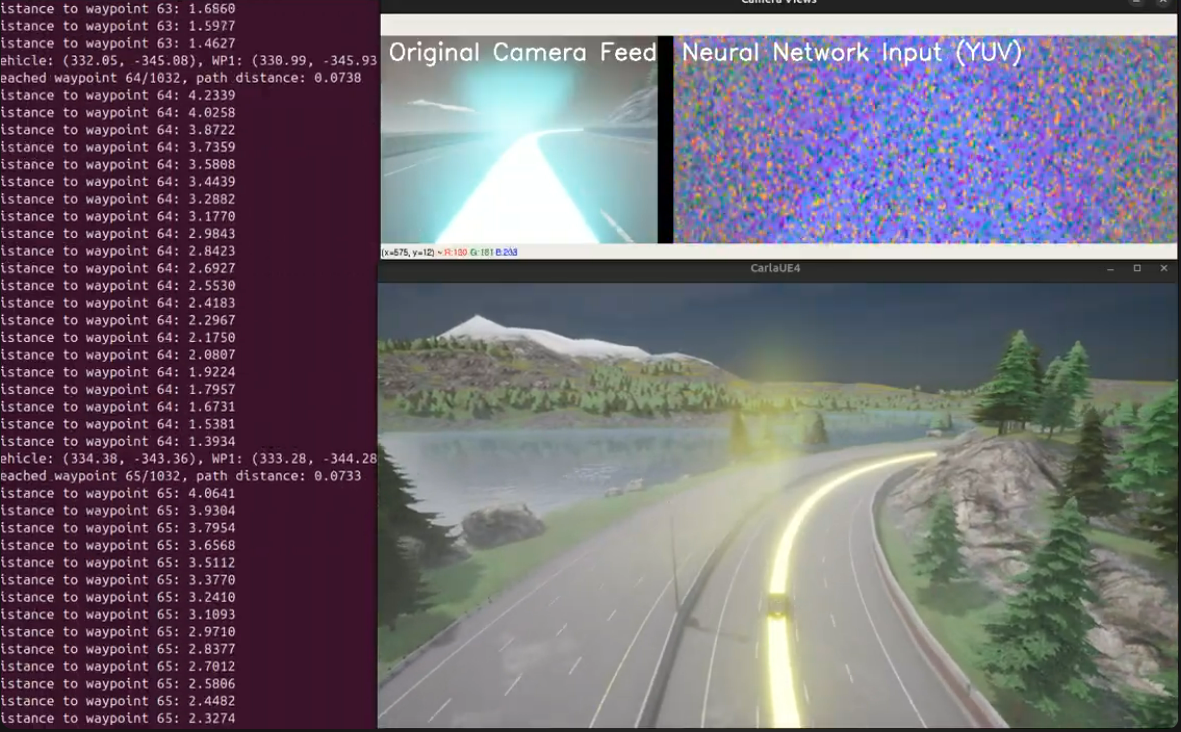
\includegraphics[width=0.75\textwidth]{Figures/Results/Exp239-30pc-noise-CNN-5-bin-bal-youtube.png}
    \caption{Experiment 239 YouTube video screenshot capture}
    \label{fig:Exp239-30pc-noise-CNN-5-bin-bal-youtube}
\end{figure}

%%%%%%%%%%%%%%%%%%%%%%%%%%%%%%%%%%%%%%%%%%%%%%%%%%%%%%%%%%%%%%%%%%%%%
% AVERAGE EUCLIDEAN DISTANCE TO CENTROIDS PRECEDING A LANE INVASION %
%%%%%%%%%%%%%%%%%%%%%%%%%%%%%%%%%%%%%%%%%%%%%%%%%%%%%%%%%%%%%%%%%%%%%

\textbf{Euclidean Distance to Centroids Preceding a Lane Invasion}
\label{res:ed_centroids_preceding_lane_invasion}

We are interested in observing if the Euclidean distance of a self-driving network softmax output to the predicted class centroid "spikes", that is presents a sharp increase, before a lane invasion is about to occur. As previously discussed, a lane invasion is defined when a vehicle's perpendicular distance to middle of the lane path is found to be greater than 0.85 units. 

Table \ref{tab:li_ed_comparison} presents average network softmax output Euclidean distance to class centroids for the last 10, 20 and 30 predictions (noting exactly one prediction is generated for every frame), where a lane invasion has occurred. Column \textbf{Exp} (integer) is the experiment ID , \textbf{Net} (string) is the network, \textbf{Noise} (integer percentage) is the percentage of pepper noise applied to the original vehicle's front facing camera image, \textbf{AvgED} (float) is the overall average Euclidean distance to predicted class centroid, \textbf{AvgED-LI-10} (float), \textbf{AvgED-LI-20} (float)  and \textbf{AvgED-LI-30} (float) is the same average, over the last 10, 20 and 30 predictions respectively, \textbf{FrCnt} (integer) is the frame count (number of predictions/frames) and \textbf{LI} (boolean) is the lane invasion boolean flag taking value T (true) when a lane invasion has occurred. Lane invasions occurred in all experiments reported in the table.

%The expectation would be that the

%%%%%%%%%%%%%%%%%%%%%%%%%%%%%%%%%%%%%%%%%%%%%%%%
% Average ED from softmax to centroids and Avg % 
% at 10, 20 and 30 frames from lane invasion   %
% selected results                             %
%%%%%%%%%%%%%%%%%%%%%%%%%%%%%%%%%%%%%%%%%%%%%%%%

% experiment 268

\begin{longtable}{@{}clcrrrrrcc@{}}
\toprule
Exp & Net & Bins & Noise & AvgED & AvgED-LI-10 & AvgED-LI-20 & AvgED-LI-30 & FrCnt & LI \\
\midrule
\endfirsthead
\toprule
Exp & Net & Bins & Noise & AvgED & AvgED-LI-10 & AvgED-LI-20 & AvgED-LI-30 & FrCnt & LI \\
\midrule
\endhead
240 & CNN & 5 & 40 & 0.6257 & 0.5616 & 0.5610 & 0.5631 & 10133 & T \\
241 & CNN & 5 & 50 & 0.6061 & 0.6215 & 0.6219 & 0.6273 & 10550 & T \\
242 & CNN & 5 & 55 & 0.5933 & 0.5135 & 0.5088 & 0.5192 & 4146 & T \\
243 & CNN & 5 & 60 & 0.5292 & 0.6206 & 0.6046 & 0.6041 & 369 & T \\
245 & ViT & 3 & 1 & 0.1063 & 0.3066 & 0.2268 & 0.1737 & 930 & T \\
246 & ViT & 3 & 2 & 0.0601 & 0.3339 & 0.2960 & 0.2088 & 144 & T \\
247 & ViT & 3 & 3 & 0.0617 & 0.3593 & 0.2924 & 0.2042 & 145 & T \\
248 & ViT & 3 & 4 & 0.0666 & 0.2934 & 0.2738 & 0.1912 & 144 & T \\
249 & ViT & 3 & 5 & 0.0697 & 0.2580 & 0.2349 & 0.1636 & 140 & T \\
250 & ViT & 3 & 7 & 0.0727 & 0.1358 & 0.2280 & 0.2591 & 271 & T \\
251 & ViT & 3 & 10 & 0.1530 & 0.3659 & 0.4113 & 0.3822 & 130 & T \\
252 & ViT & 3 & 20 & 0.2156 & 0.5062 & 0.4387 & 0.3874 & 108 & T \\
253 & ViT & 3 & 30 & 0.3234 & 0.5033 & 0.4594 & 0.4011 & 90 & T \\
254 & ViT & 3 & 40 & 0.4130 & 0.3171 & 0.3938 & 0.4251 & 58 & T \\
255 & ViT & 3 & 50 & 0.5513 & 0.5834 & 0.5582 & 0.5628 & 34 & T \\
256 & ViT & 5 & 10 & 0.4051 & 0.5901 & 0.5571 & 0.4842 & 164 & T \\
257 & ViT & 5 & 20 & 0.5415 & 0.6642 & 0.6754 & 0.6732 & 101 & T \\
258 & ViT & 5 & 30 & 0.5588 & 0.6995 & 0.6623 & 0.6020 & 120 & T \\
259 & ViT & 5 & 40 & 0.6238 & 0.7005 & 0.6296 & 0.6227 & 157 & T \\
260 & ViT & 5 & 50 & 0.7479 & 0.7522 & 0.7637 & 0.7658 & 114 & T \\
261 & ViT & 5 & 60 & 0.7627 & 0.7671 & 0.7598 & 0.7571 & 34 & T \\
\bottomrule
\caption{Comparison of Overall and Last 10, 20, 30 Predictions Euclidean Distance to Predicted Class Centroids for Experiments where Lane Invasion Occurred}
\label{tab:li_ed_comparison}
\end{longtable}


In Table \ref{tab:li_ed_comparison} the average Euclidean distance to predicted class centroid for the last 10, 20 and 30 predictions is examined, for experiments that resulted in lane invasions.

Table \ref{tab:experiment_stats} reports key metrics—average path distance (AvgPD), Euclidean distance (AvgED), Bhattacharyya distance (AvgBD), histogram intersection (AvgHI), KL divergence (AvgKL), frame count (FrCnt), and lane invasion status (LI)—across 27 experiments. Lane invasions (LI = T) occurred at noise levels of 40–60\% for CNN (5 bins) and 1–60\% for ViT (3/5 bins), with increased AvgED and AvgKL signaling prediction instability. Figure \ref{fig:combined_cnn_5bin_vit_3bin_vit_5bin_noise_distance_metrics} shows normalized metrics against noise (0, 10, 20, 30, 40, 50\%), with shaded regions indicating LI = T thresholds (e.g., Noise 40 for CNN, 5 bins; Noise 10 for ViT, 3/5 bins), highlighting metric degradation during invasions. Table~\ref{tab:youtube_links} provides YouTube video links for select experiments (e.g., Exp 261, ViT, 5 bins, 60\% noise), showing evidence of lane invasions.

Table~\ref{tab:li_ed_comparison} analyzes 21 LI = T experiments (Exps 240–243, 245–261), comparing the overall average Euclidean distance (AvgED) to averages for the last 10, 20, and 30 predictions (AvgED-LI-10, AvgED-LI-20, AvgED-LI-30), alongside noise and frame counts.

For CNN (5 bins), AvgED-LI-10 varies relative to AvgED (e.g., 0.5616 vs. 0.6257 for Exp 240; 0.6215 vs. 0.6061 for Exp 241), with AvgED-LI-20 and AvgED-LI-30 showing similar variability (e.g., 0.5610, 0.5631 for Exp 240; 0.6046, 0.6041 for Exp 243), suggesting inconsistent prediction errors near invasions.

For ViT (3 bins), AvgED-LI-10 is often higher than AvgED at low noise (e.g., 0.3066 vs. 0.1063 for Exp 245, Noise 1\%), but AvgED-LI-20 and AvgED-LI-30 decrease (e.g., 0.2268, 0.1737), indicating transient errors in the final 10 frames that stabilize over longer windows. At higher noise (e.g., Exp 252, Noise 20\%), AvgED-LI-10 remains high (0.5062), with AvgED-LI-20 and AvgED-LI-30 slightly lower (0.4387, 0.3874), suggesting sustained degradation.

For ViT (5 bins), AvgED-LI-10 consistently exceeds AvgED (e.g., 0.6642 vs. 0.5415 for Exp 257, Noise 20\%), with AvgED-LI-20 and AvgED-LI-30 varying (e.g., 0.6754, 0.6732 for Exp 257; 0.7598, 0.7571 for Exp 261), reflecting persistent prediction errors.

These findings highlight ViT's greater sensitivity to noise, with earlier lane invasions (Noise 1\% for 3 bins) and larger prediction errors in the final 10–30 frames compared to CNN (Noise 40\%), critical for assessing safety in noisy environments.

%%%%%%%%%%%%%%
% CONCLUSION %
%%%%%%%%%%%%%%

\section{Conclusion}

The work presented in this section demonstrates practical applications for quantifying uncertainty using the softmax space and softmax output distance to centroids. By first training two distinct neural network architectures, CNNs and ViTs, with synthetic datasets generated in a simulated environment presenting realistic conditions, the steering task was learned such that the simulated vehicles were able to drive around a figure of 8 circuit, where the lane to be driven in was segmented, without invading a neighbouring lane. Telemetry was taken to characterize acceptable driving. Noise was then added incrementally to front-facing vehicle camera images, before the noise-added images were presented to the steering network. 5 and 3 bin trained models were used, e.g. to predict steering classes "left", "straight" and "right", and prediction distances to class centroids recorded for all predictions. Lane invasions were determined by the distance of the vehicle to the middle path.

\section{Future Work}

The practical application illustrated in this work could be applied to any autonomous system relying on classification or regression for decision making. The use of Vision Language Models offers interesting research paths, be it in studying the softmax space and distances to centroids, or leveraging other metrics e.g. cosine similarity in the embedding space, to quantify and ultimately avoid hallucinations and bias.
